% !TeX root = 0_main.tex
\documentclass[a4paper,14pt,oneside,openany]{memoir}

%%% Задаем поля, отступы и межстрочный интервал %%%

\usepackage[left=30mm, right=15mm, top=20mm, bottom=20mm]{geometry} % Пакет geometry с аргументами для определения полей
\pagestyle{plain} % Убираем стандарные для данного класса верхние колонтитулы с заголовком текущей главы, оставляем только номер страницы снизу по центру
\parindent=1.25cm % Абзацный отступ 1.25 см, приблизительно равно пяти знакам, как по ГОСТ
\usepackage{indentfirst} % Добавляем отступ к первому абзацу
%\linespread{1.3} % Межстрочный интервал (наиболее близко к вордовскому полуторному) - тут вместо этого используется команда OnehalfSpacing*

%%% Задаем языковые параметры и шрифт %%%

\usepackage[english, russian]{babel}                % Настройки для русского языка как основного в тексте
\babelfont{rm}{Times New Roman}                     % TMR в качестве базового roman-щрифта

%%% Задаем стиль заголовков и подзаголовков в тексте %%%

\setsecnumdepth{subsection} % Номера разделов считать до третьего уровня включительно, т.е. нумеруются только главы, секции, подсекции
\renewcommand*{\chapterheadstart}{} % Переопределяем команду, задающую отступ над заголовком, чтобы отступа не было
\renewcommand*{\printchaptername}{} % Переопределяем команду, печатающую слово "Глава", чтобы оно не печалось
%\renewcommand*{\printchapternum}{} % То же самое для номера главы - тут не надо, номер главы оставляем
\renewcommand*{\chapnumfont}{\normalfont\bfseries} % Меняем стиль шрифта для номера главы: нормальный размер, полужирный
\renewcommand*{\afterchapternum}{\hspace{1em}} % Меняем разделитель между номером главы и названием
\renewcommand*{\printchaptertitle}{\normalfont\bfseries\centering\MakeUppercase} % Меняем стиль написания для заголовка главы: нормальный размер, полужирный, центрированный, заглавными буквами
\setbeforesecskip{20pt} % Задаем отступ перед заголовком секции
\setaftersecskip{20pt} % Ставим такой же отступ после заголовка секции
\setsecheadstyle{\raggedright\normalfont\bfseries} % Меняем стиль написания для заголовка секции: выравнивание по правому краю без переносов, нормальный размер, полужирный
\setbeforesubsecskip{20pt} % Задаем отступ перед заголовком подсекции
\setaftersubsecskip{20pt} % Ставим такой же отступ после заголовка подсекции
\setsubsecheadstyle{\raggedright\normalfont\bfseries}  % Меняем стиль написания для заголовка подсекции: выравнивание по правому краю без переносов, нормальный размер, полужирный

%%% Задаем параметры оглавления %%%

\addto\captionsrussian{\renewcommand\contentsname{Содержание}} % Меняем слово "Оглавление" на "Содержание"
\setrmarg{2.55em plus1fil} % Запрещаем переносы слов в оглавлении
%\setlength{\cftbeforechapterskip}{0pt} % Эта команда убирает интервал между заголовками глав - тут не надо, так красивее смотрится
\renewcommand{\aftertoctitle}{\afterchaptertitle \vspace{-\cftbeforechapterskip}} % Делаем отступ между словом "Содержание" и первой строкой таким же, как у заголовков глав
%\renewcommand*{\chapternumberline}[1]{} % Делаем так, чтобы номер главы не печатался - тут не надо
\renewcommand*{\cftchapternumwidth}{1.5em} % Ставим подходящий по размеру разделитель между номером главы и самим заголовком
\renewcommand*{\cftchapterfont}{\normalfont\MakeUppercase} % Названия глав обычным шрифтом заглавными буквами
\renewcommand*{\cftchapterpagefont}{\normalfont} % Номера страниц обычным шрифтом
\renewcommand*{\cftchapterdotsep}{\cftdotsep} % Делаем точки до номера страницы после названий глав
\renewcommand*{\cftdotsep}{1} % Задаем расстояние между точками
\renewcommand*{\cftchapterleader}{\cftdotfill{\cftchapterdotsep}} % Делаем точки стандартной формы (по умолчанию они "жирные")
\maxtocdepth{subsection} % В оглавление попадают только разделы первыхтрех уровней: главы, секции и подсекции

%%% Выравнивание и переносы %%%

%% http://tex.stackexchange.com/questions/241343/what-is-the-meaning-of-fussy-sloppy-emergencystretch-tolerance-hbadness
%% http://www.latex-community.org/forum/viewtopic.php?p=70342#p70342
\tolerance 1414
\hbadness 1414
\emergencystretch 1.5em                             % В случае проблем регулировать в первую очередь
\hfuzz 0.3pt
\vfuzz \hfuzz
%\dbottom
%\sloppy                                            % Избавляемся от переполнений
\clubpenalty=10000                                  % Запрещаем разрыв страницы после первой строки абзаца
\widowpenalty=10000                                 % Запрещаем разрыв страницы после последней строки абзаца
\brokenpenalty=4991                                 % Ограничение на разрыв страницы, если строка заканчивается переносом

%%% Объясняем компилятору, какие буквы русского алфавита можно использовать в перечислениях (подрисунках и нумерованных списках) %%%
%%% По ГОСТ нельзя использовать буквы ё, з, й, о, ч, ь, ы, ъ %%%
%%% Здесь также переопределены заглавные буквы, хотя в принципе они в документе не используются %%%

\makeatletter
    \def\russian@Alph#1{\ifcase#1\or
       А\or Б\or В\or Г\or Д\or Е\or Ж\or
       И\or К\or Л\or М\or Н\or
       П\or Р\or С\or Т\or У\or Ф\or Х\or
       Ц\or Ш\or Щ\or Э\or Ю\or Я\else\xpg@ill@value{#1}{russian@Alph}\fi}
    \def\russian@alph#1{\ifcase#1\or
       а\or б\or в\or г\or д\or е\or ж\or
       и\or к\or л\or м\or н\or
       п\or р\or с\or т\or у\or ф\or х\or
       ц\or ш\or щ\or э\or ю\or я\else\xpg@ill@value{#1}{russian@alph}\fi}
\makeatother

%%% Задаем параметры оформления рисунков и таблиц %%%

\usepackage{graphicx, caption, subcaption} % Подгружаем пакеты для работы с графикой и настройки подписей
\graphicspath{{images/}} % Определяем папку с рисунками
\captionsetup[figure]{font=small, width=\textwidth, name=Рисунок, justification=centering} % Задаем параметры подписей к рисункам: маленький шрифт (в данном случае 12pt), ширина равна ширине текста, полнотекстовая надпись "Рисунок", выравнивание по центру
\captionsetup[subfigure]{font=small} % Индексы подрисунков а), б) и так далее тоже шрифтом 12pt (по умолчанию делает еще меньше)
\captionsetup[table]{singlelinecheck=false,font=small,width=\textwidth,justification=justified} % Задаем параметры подписей к таблицам: запрещаем переносы, маленький шрифт (в данном случае 12pt), ширина равна ширине текста, выравнивание по ширине
\captiondelim{ --- } % Разделителем между номером рисунка/таблицы и текстом в подписи является длинное тире
\setkeys{Gin}{width=\textwidth} % По умолчанию размер всех добавляемых рисунков будет подгоняться под ширину текста
\renewcommand{\thesubfigure}{\asbuk{subfigure}} % Нумерация подрисунков строчными буквами кириллицы
%\setlength{\abovecaptionskip}{0pt} % Отбивка над подписью - тут не меняем
%\setlength{\belowcaptionskip}{0pt} % Отбивка под подписью - тут не меняем
\usepackage[section]{placeins} % Объекты типа float (рисунки/таблицы) не вылезают за границы секциии, в которой они объявлены

%%% Задаем параметры ссылок и гиперссылок %%% 

\usepackage{hyperref}                               % Подгружаем нужный пакет
\hypersetup{
    colorlinks=true,                                % Все ссылки и гиперссылки цветные
    linktoc=all,                                    % В оглавлении ссылки подключатся для всех отображаемых уровней
    linktocpage=true,                               % Ссылка - только номер страницы, а не весь заголовок (так выглядит аккуратнее)
    linkcolor=red,                                  % Цвет ссылок и гиперссылок - красный
    citecolor=red                                   % Цвет цитировний - красный
}

%%% Настраиваем отображение списков %%%

\usepackage{enumitem}                               % Подгружаем пакет для гибкой настройки списков
\renewcommand*{\labelitemi}{\normalfont{--}}        % В ненумерованных списках для пунктов используем короткое тире
\makeatletter
    \AddEnumerateCounter{\asbuk}{\russian@alph}     % Объясняем пакету enumitem, как использовать asbuk
\makeatother
\renewcommand{\labelenumii}{\asbuk{enumii})}        % Кириллица для второго уровня нумерации
\renewcommand{\labelenumiii}{\arabic{enumiii})}     % Арабские цифры для третьего уровня нумерации
\setlist{noitemsep, leftmargin=*}                   % Убираем интервалы между пунками одного уровня в списке
\setlist[1]{labelindent=\parindent}                 % Отступ у пунктов списка равен абзацному отступу
\setlist[2]{leftmargin=\parindent}                  % Плюс еще один такой же отступ для следующего уровня
\setlist[3]{leftmargin=\parindent}                  % И еще один для третьего уровня

%%% Счетчики для нумерации объектов %%%

\counterwithout{figure}{chapter}                    % Сквозная нумерация рисунков по документу
\counterwithout{equation}{chapter}                  % Сквозная нумерация математических выражений по документу
\counterwithout{table}{chapter}                     % Сквозная нумерация таблиц по документу

%%% Реализация библиографии пакетами biblatex и biblatex-gost с использованием движка biber %%%

\usepackage{csquotes} % Пакет для оформления сложных блоков цитирования (biblatex рекомендует его подключать)
\usepackage[%
backend=biber,                                      % Движок
bibencoding=utf8,                                   % Кодировка bib-файла
sorting=none,                                       % Настройка сортировки списка литературы
style=gost-numeric,                                 % Стиль цитирования и библиографии по ГОСТ
language=auto,                                      % Язык для каждой библиографической записи задается отдельно
autolang=other,                                     % Поддержка многоязычной библиографии
sortcites=true,                                     % Если в квадратных скобках несколько ссылок, то отображаться будут отсортированно
movenames=false,                                    % Не перемещать имена, они всегда в начале библиографической записи
maxnames=5,                                         % Максимальное отображаемое число авторов
minnames=3,                                         % До скольки сокращать число авторов, если их больше максимума
doi=false,                                          % Не отображать ссылки на DOI
isbn=false,                                         % Не показывать ISBN, ISSN, ISRN
]{biblatex}[2016/09/17]
\DeclareDelimFormat{bibinitdelim}{}                 % Убираем пробел между инициалами (Иванов И.И. вместо Иванов И. И.)
\addbibresource{./biba.bib}                           % Определяем файл с библиографией

%%% Скрипт, который автоматически подбирает язык (и, следовательно, формат) для каждой библиографической записи %%%
%%% Если в названии работы есть кириллица - меняем значение поля langid на russian %%%
%%% Все оставшиеся пустые места в поле langid заменяем на english %%%

\DeclareSourcemap{
  \maps[datatype=bibtex]{
    \map{
        \step[fieldsource=title, match=\regexp{^\P{Cyrillic}*\p{Cyrillic}.*}, final]
        \step[fieldset=langid, fieldvalue={russian}]
    }
    \map{
        \step[fieldset=langid, fieldvalue={english}]
    }
  }
}

%%% Прочие пакеты для расширения функционала %%%

\usepackage{longtable,ltcaption}                    % Длинные таблицы
\usepackage{multirow,makecell}                      % Улучшенное форматирование таблиц
\usepackage{booktabs}                               % Еще один пакет для красивых таблиц
\usepackage{soulutf8}                               % Поддержка переносоустойчивых подчёркиваний и зачёркиваний
\usepackage{icomma}                                 % Запятая в десятичных дробях
\usepackage{hyphenat}                               % Для красивых переносов
\usepackage{textcomp}                               % Поддержка "сложных" печатных символов типа значков иены, копирайта и т.д.
\usepackage[version=4]{mhchem}                      % Красивые химические уравнения
\usepackage{amsmath}                                % Усовершенствование отображения математических выражений 

%%% Вставляем по очереди все содержательные части документа %%%

\begin{document}

\thispagestyle{empty}

\begin{center}
    МИНИСТЕРСТВО НАУКИ И ВЫСШЕГО ОБРАЗОВАНИЯ \\ РОССИЙСКОЙ ФЕДЕРАЦИИ

    \vspace{20pt}

    Федеральное государственное автономное \\ образовательное учреждение высшего образования \\
    "<Национальный исследовательский университет ИТМО"> \\
    (Университет ИТМО)

    \vspace{20pt}

    Факультет систем управления и робототехники \\
\end{center}

\vfill

\begin{center}
    ВЫПУСКНАЯ КВАЛИФИКАЦИОННАЯ РАБОТА \\  
    GRADUATION THESIS \\

    \vspace{20pt}

    по теме: \\
    \uppercase{Исследование алгоритмов компьютерного зрения для отслеживания подводных объектов}
\end{center}

\vfill

    \noindent Студент: \\
    \textit{Группа № R34372 \hfill Нгуен Тоан}

    \vspace{20pt}

    \noindent Руководитель: \\
    \textit{Доцент, кандидат технических наук \hfill Шаветов Сергей Васильевич}

\vfill

\begin{center}
    Санкт-Петербург 2025
\end{center}                                     % Титульник

\newpage % Переходим на новую страницу
\setcounter{page}{2} % Начинаем считать номера страниц со второй
\OnehalfSpacing* % Задаем полуторный интервал текста (в титульнике одинарный, поэтому команда стоит после него)

\tableofcontents*                                   % Автособираемое оглавление

\chapter*{Introduction}
\addcontentsline{toc}{chapter}{Введение}
\label{ch:intro}

Computer vision is one of the most rapidly developing fields in modern artificial intelligence, with applications spanning a wide range of tasks, from autonomous driving to medical diagnostics and industrial automation systems. One of the critical and complex challenges researchers face is object tracking in underwater environments. Underwater conditions are characterized by complex optical distortions, low image contrast, uneven lighting, and various noise effects, which significantly complicate the process of video data processing and analysis.

The relevance of this topic is driven by the need to create reliable monitoring systems and manage underwater robotic complexes, as well as to improve methods for marine security and scientific research of ocean resources. The application of modern machine learning and neural network techniques to solve the problem of object tracking in underwater environments allows for enhanced accuracy and robustness of algorithms, which opens up new opportunities for the practical implementation of developed solutions.

The goal of this work is to investigate and develop computer vision algorithms capable of efficiently tracking underwater objects under significant visual distortions. To achieve this goal, several tasks need to be accomplished: conducting an analytical review of existing methods and algorithms used for tracking objects in complex visual conditions; preparing and analyzing the UOT100 dataset, which contains over 100 video sequences under various underwater conditions; evaluating the effectiveness of classical machine learning methods compared to modern neural network approaches, including algorithms based on correlation filters and Siamese networks; and developing software in Python using libraries such as OpenCV, PyTorch, and TensorFlow to implement and compare the selected algorithms.

The structure of the work includes an introduction that justifies the relevance of the topic and sets the research objectives, an overview of existing solutions, a theoretical part dedicated to studying the principles of computer vision algorithms, a description of the experimental setup and analysis conducted, as well as conclusions and recommendations for further development of the topic. The research carried out will not only identify the strengths and weaknesses of existing approaches but also propose directions for their improvement in the context of underwater applications. 

Thus, the work aims to address practical problems related to improving the efficiency of object tracking systems in extreme conditions, which is of great significance for the development of autonomous underwater technologies and the implementation of new solutions in marine safety and monitoring.

\endinput                                     % Введение
\chapter{Problem statement}
\label{ch:chap1}

Tracking underwater objects, which refers to the continuous and accurate estimation of a target's position within a video sequence captured underwater, is a critical task with significant implications for marine applications. These applications span across environmental monitoring, resource development, and ecological protection \cite{qiu2024boundary}, where precise tracking can aid in assessing marine ecosystems, monitoring aquatic life, and ensuring the sustainability of ocean resources. However, the unique characteristics of the underwater environment introduce substantial challenges that complicate the task of object tracking in this setting.

One of the foremost challenges is the issue of \textbf{water turbidity and blurring effects}. Underwater optical images are frequently affected by turbidity, which results in significant blurring and fog. This occurs due to the absorption and scattering of light by seawater and various suspended particles, including minerals, salt, sand, and plankton \cite{zhou2024real, elmezain2025advancing, bhadouriaunderwater}. The turbid nature of water severely limits visibility, introducing haze that further complicates the clarity of captured images. Additionally, turbulence in the water flow can cause motion blur, which further disrupts the tracking process and reduces the precision of object localization \cite{bhadouriaunderwater}.

% example water turbidity and blurring effects
\begin{figure}[ht]
    \centering
    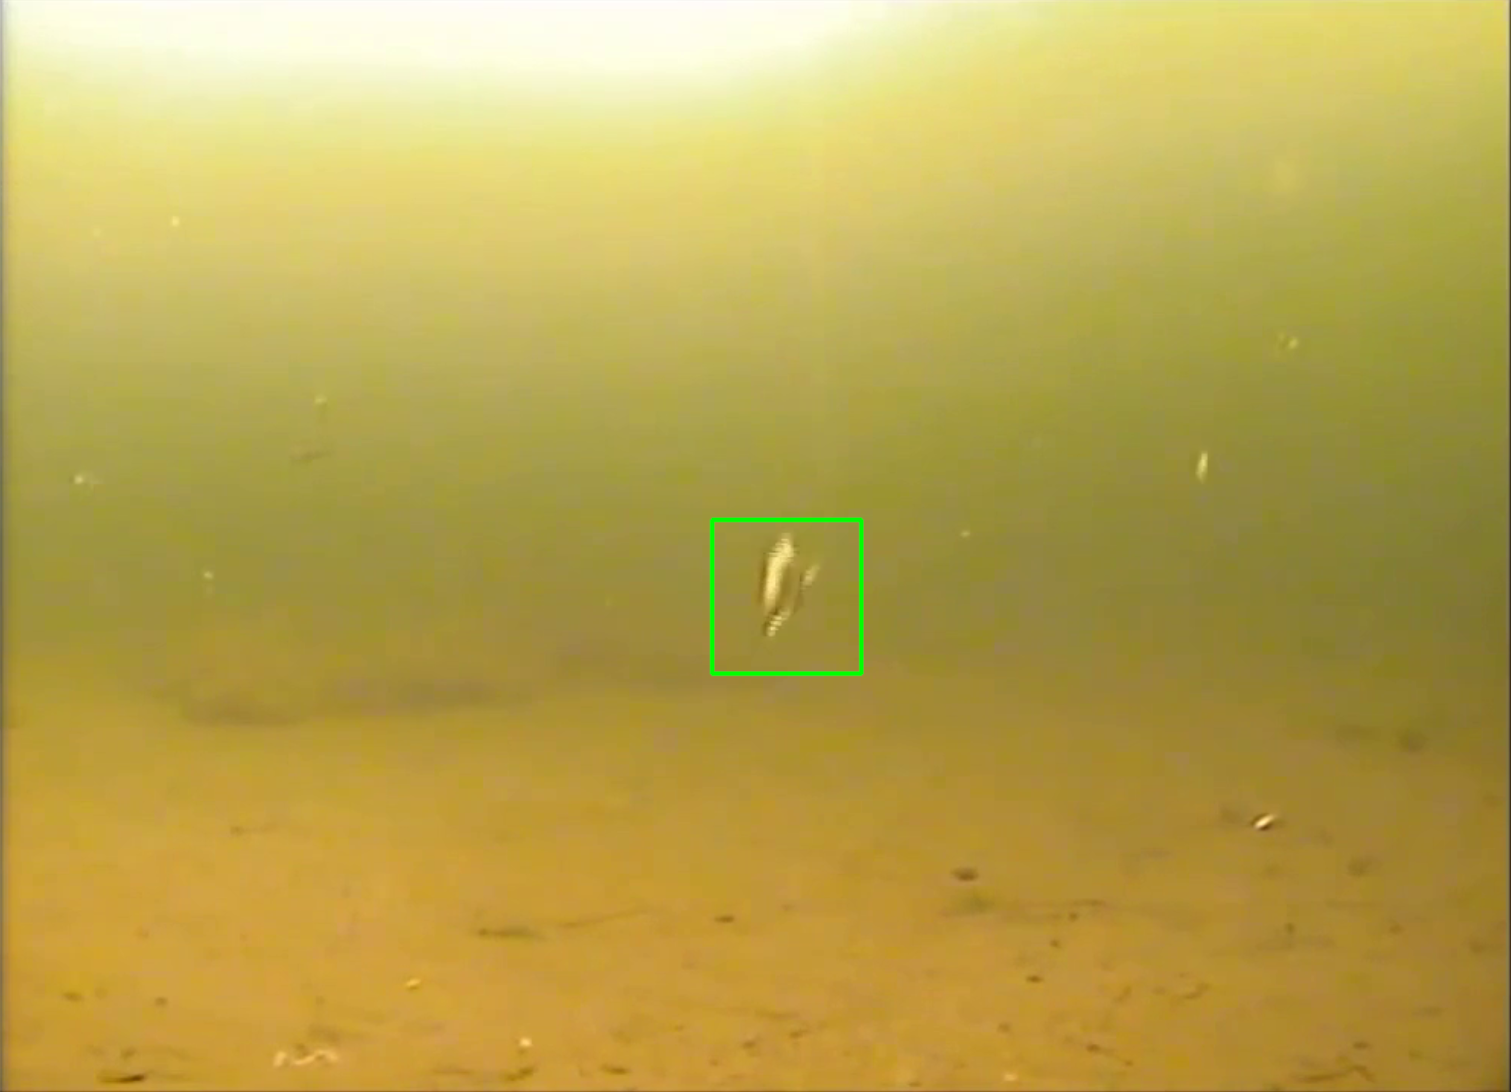
\includegraphics[width=0.8\textwidth]{images/water turbidity and blurring effects.png}
    \caption{Example of water turbidity and blurring effects. Source: UOT100 dataset \cite{kezebou2019underwater}.}
    \label{fig:turbidity}
\end{figure}


Another obstacle faced in underwater tracking is \textbf{color attenuation and light scattering}. As light travels through water, different wavelengths are absorbed at varying rates, with red light being absorbed more rapidly than other wavelengths \cite{elmezain2025advancing}. This phenomenon leads to the attenuation of color, which distorts the natural hues of objects and affects the overall image quality. The scattering of light by suspended particles further diminishes light intensity and alters its direction, resulting in color distortion that can make it even more difficult to distinguish between different objects. This attenuation of color and reduction in light intensity contribute to the overall decolorization of underwater scenes, posing a significant challenge for accurate object tracking \cite{elmezain2025advancing, bhadouriaunderwater, rout2019walsh}.
% Bluelike
\begin{figure}[ht]
    \centering
    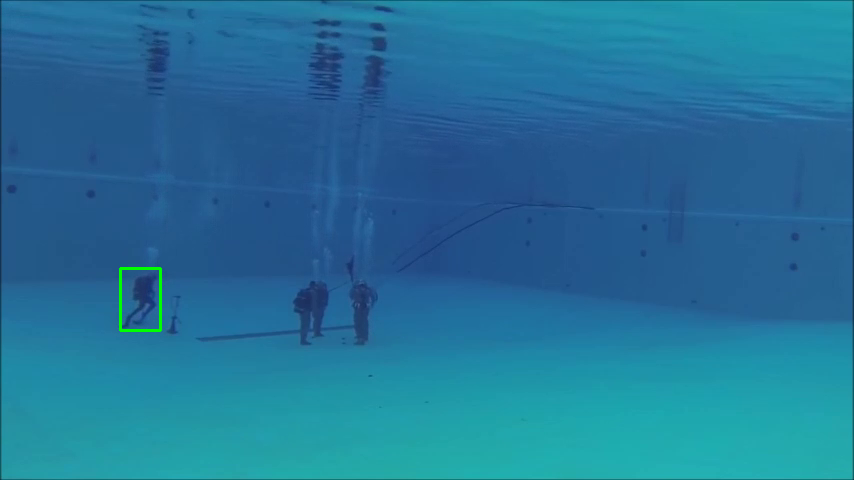
\includegraphics[width=0.9\textwidth]{images/color attenuation and light scattering.png}
    \caption{Example of color attenuation and light scattering. Source: UOT100 dataset \cite{kezebou2019underwater}.}
    \label{fig:color attenuation}
\end{figure}

In addition to these optical challenges, \textbf{low-contrast targets and occlusion} are persistent problems in underwater environments. Low visibility, low contrast, and low light intensity are common characteristics of underwater images, making it particularly difficult to discern objects and extract meaningful features for tracking \cite{zhou2024real, bhadouriaunderwater}. Moreover, many marine species exhibit camouflage, blending seamlessly with their surroundings, which complicates the process of segmentation and accurate identification \cite{elmezain2025advancing}. Furthermore, occlusion, where one object partially or fully obscures another, presents a substantial problem. This can significantly hinder the ability to maintain a consistent track of the target, especially in dynamic environments where objects frequently move in and out of view \cite{zhou2024real, elmezain2025advancing, mathias2022occlusion}.

% example low-contrast targets and occlusion
\begin{figure}[ht]
    \centering
    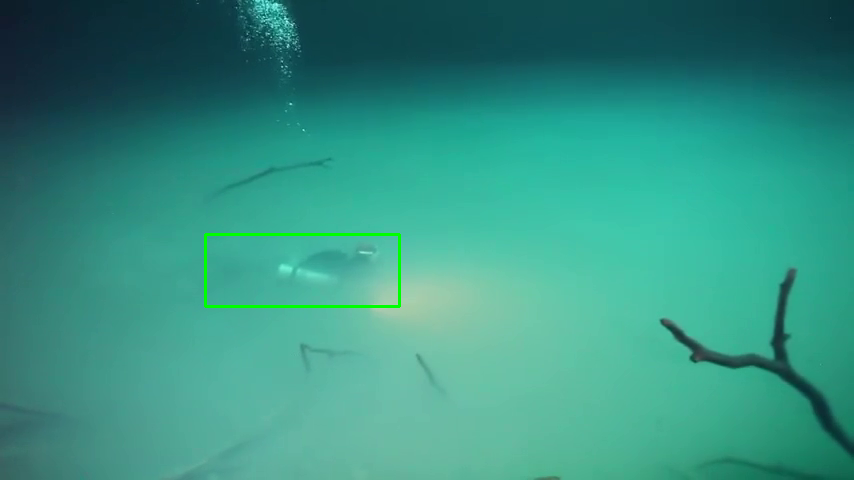
\includegraphics[width=0.8\textwidth]{images/CenoteAngelita.png}
    \caption{Example of low-contrast targets and occlusion. Source: UOT100 dataset \cite{kezebou2019underwater}.}
    \label{fig:low-contrast}
\end{figure}

The underwater environment is also characterized by \textbf{dynamic backgrounds with similar-looking objects}, adding another layer of complexity. Marine organisms exhibit a wide range of sizes and shapes, often appearing in dense clusters or schools, such as schools of fish. The presence of these similar-looking objects in the background can lead to confusion, as tracking algorithms may mistakenly identify these objects as the target, causing errors and drift in the tracking process \cite{zhang2024webuot}. The complexity and dynamic nature of the underwater scene further exacerbate the challenges faced by tracking algorithms.
% example dynamic backgrounds with similar-looking objects
\begin{figure}[ht]
    \centering
    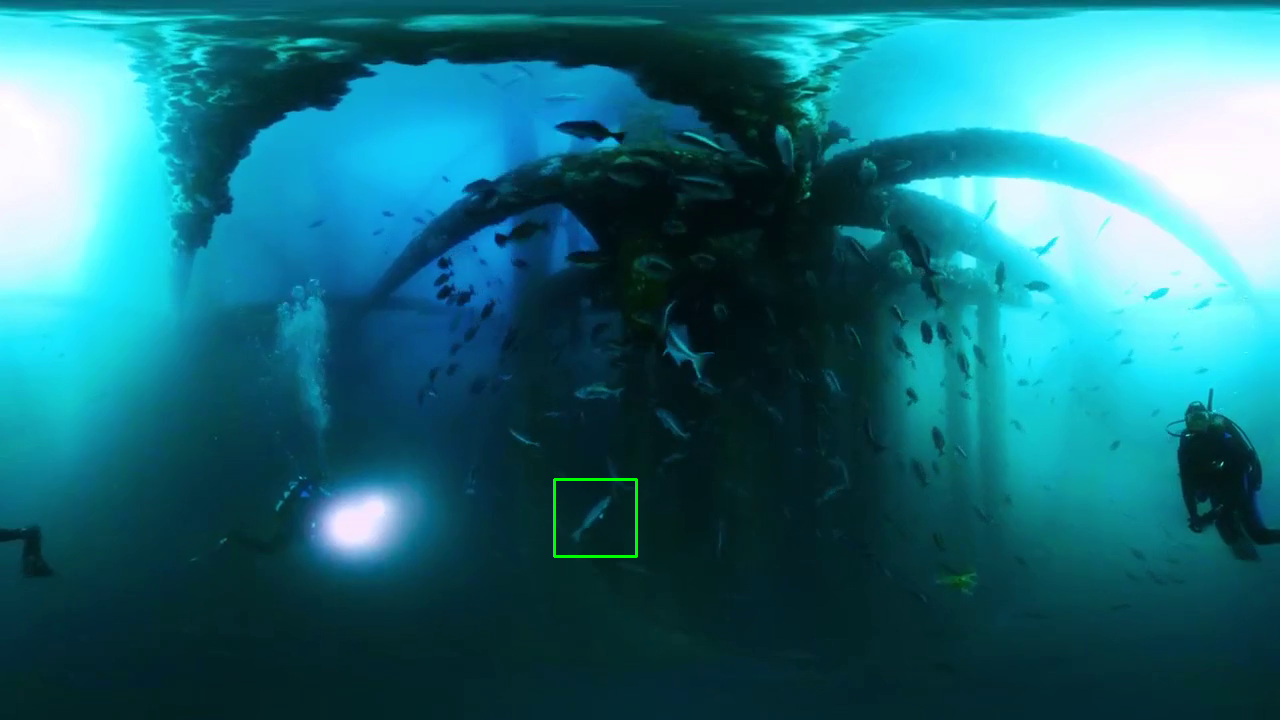
\includegraphics[width=0.8\textwidth]{images/Diving360Degree2.png}
    \caption{Example of dynamic backgrounds with similar-looking objects. Source: UOT100 dataset \cite{kezebou2019underwater}.}
    \label{fig:dynamic backgrounds}
\end{figure}

Traditional object tracking methods, primarily designed and optimized for open-air environments, struggle to perform effectively in underwater settings \cite{elmezain2025advancing}. These conventional methods are not robust enough to handle the significant domain shifts introduced by the optical properties of water, such as color distortion, image blur, and light scattering \cite{elmezain2025advancing}. Moreover, mainstream tracking models can be computationally expensive, often requiring high computational power that may not be available on resource-constrained underwater edge devices \cite{qiu2024boundary}. The inherent challenges of target feature distortion and contrast attenuation in underwater scenes can further undermine the ability of general tracking algorithms to differentiate between the target and its background, reducing their reliability. Therefore, specialized tracking models that take into account the unique characteristics of the underwater environment, along with underwater-specific datasets, are essential for improving the accuracy and reliability of object tracking in such challenging conditions \cite{elmezain2025advancing}.

\endinput                                     % Первая глава
\chapter{Overview of Existing Solutions}
\label{ch:chap2}

\section{Correlation Filter-Based Tracking Methods}
\label{sec:tradi}

% introduce
Correlation Filter (CF)-Based Tracking has emerged as a prominent approach in visual object tracking, known for achieving a good balance between tracking accuracy and speed \cite{feng2019dynamic}. These methods utilize a dynamic model to track the same target across consecutive video frames \cite{du2021overview}. The core idea revolves around learning a correlation filter in the frequency domain to efficiently locate the target in subsequent frames \cite{zhao2020correlation}.

% Step by step
\begin{figure}[h]
    \centering
    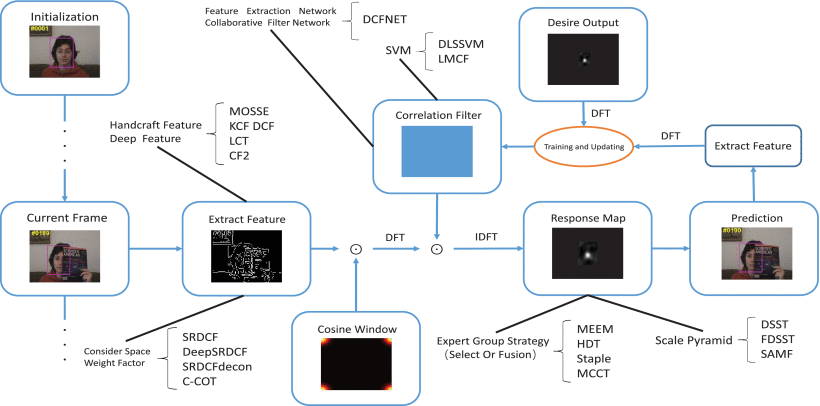
\includegraphics[width=1\linewidth]{images/General framework for correlation-filter-based object tracking.png}
    \caption{General framework for correlation-filter-based object tracking \cite{du2021overview}}
    \label{fig:CF-general-framework}
\end{figure}

The general framework for correlation filter-based object tracking typically involves the following steps \cite{du2021overview}\cite{zhao2020correlation}:
\begin{enumerate}
    \item \textbf{Feature Extraction}: In the initial frame, features are extracted from an image block at the target's location  \cite{du2021overview} \cite{zhao2020correlation}. These features can include handcrafted features like grayscale, Histogram of Oriented Gradients (HOG) \cite{zhao2020correlation}\cite{du2021overview}, and color names (CN) \cite{lin2024motion}, or deep features extracted from Convolutional Neural Networks (CNNs) \cite{du2021overview}\cite{zhao2020correlation}\cite{lin2024motion} . A cosine window is often applied to reduce boundary effects \cite{du2021overview}.

    \item \textbf{Filter Training:} A correlation filter is learned based on the extracted features and a desired output, often a Gaussian-shaped response map centered at the target \cite{feng2019dynamic}\cite{du2021overview} . This learning process aims to create a filter that produces a strong correlation response when convolved with the target and a weak response elsewhere \cite{qiu2024boundary}\cite{du2021overview}. Techniques like the Minimum Output Sum of Squared Error (MOSSE) algorithm represent early and straightforward approaches to filter learning \cite{feng2019dynamic} \cite{du2021overview} \cite{zhao2020correlation}. Kernel Correlation Filters (KCF) further enhance this by utilizing a cyclic matrix to construct training samples and employing kernel functions to handle non-linear features \cite{du2021overview}\cite{zhao2020correlation}\cite{lin2024motion}. Dual Correlation Filters (DCF) represent another early development \cite{du2021overview}.

    \item \textbf{Target Localization:} In subsequent frames, a search window centered around the previous target location is cropped, and features are extracted \cite{zhao2020correlation}. The learned correlation filter is then convolved with these features to generate a response map \cite{du2021overview}\cite{zhao2020correlation}. The location of the maximum response in this map indicates the new position of the target \cite{du2021overview}\cite{zhao2020correlation}. The response map's characteristics, such as its peak value and shape, can also be used for tasks like failure detection \cite{lin2024motion}.

    \item \textbf{Filter Update:} To adapt to changes in the target's appearance and the environment, the correlation filter is typically updated online with new information from the tracked target in the current frame \cite{qiu2024boundary}\cite{du2021overview}\cite{zhao2020correlation}. The learning rate of this update can be adaptively determined based on tracking reliability \cite{du2021overview}.
\end{enumerate}

% Categorization
Correlation filter-based object tracking methods have undergone significant advancements and can be categorized based on several key characteristics \cite{du2021overview}. Early approaches utilized categorized features such as grayscale information, exemplified by the Minimum Output Sum of Squared Error (MOSSE) tracker \cite{feng2019dynamic}\cite{zhao2020correlation}\cite{lin2024motion}. Subsequent developments incorporated more sophisticated handcrafted features like Histogram of Oriented Gradients (HOG) and color names \cite{elmezain2025advancing}\cite{zhang2024webuot}\cite{feng2019dynamic}\cite{lin2024motion}. The integration of deep convolutional neural network (CNN) features has further enhanced performance by providing robust and discriminative representations \cite{feng2019dynamic}\cite{du2021overview}\cite{lin2024motion}. Some trackers leverage a combination of handcrafted and deep features to capitalize on their complementary strengths \cite{zhang2024webuot}\cite{du2021overview}\cite{lin2024motion}.

Another crucial categorization factor is the consideration of the spatial context through space weight factors. Spatially Regularized Discriminative Correlation Filters (SRDCF) were introduced to mitigate boundary effects by penalizing filter coefficients outside the target region \cite{du2021overview}\cite{feng2019dynamic}\cite{lin2024motion}. Variants like DeepSRDCF combine SRDCF with deep features \cite{feng2019dynamic}\cite{du2021overview}, and CSRDCF incorporates channel and spatial reliability \cite{feng2019dynamic}\cite{du2021overview}\cite{zhao2020correlation}. Dynamic Saliency-Aware Regularized CF Tracking (DSAR-CF) refines spatial regularization by integrating object saliency information, allowing the weight map to adapt to shape variations \cite{feng2019dynamic}\cite{du2021overview}\cite{lin2024motion}.
Scale factors represent another important category. Discriminative Scale Space Tracking (DSST) decouples translation and scale estimation to accurately determine the object's size \cite{zhang2024webuot}\cite{feng2019dynamic}\cite{lin2024motion}.

Expert strategies involve utilizing multiple filters or cues and selecting the most reliable one for tracking. Multiexpert Entropy Minimization (MEEM) based on Support Vector Machines (SVM) is an example of this approach \cite{du2021overview}\cite{srigowri2022enhancing}. Methods employing decision-level fusion also fall under this category, combining the outputs of multiple experts based on different features or filter types \cite{lin2024motion}\cite{elmezain2025advancing}. Large Margin Object Tracking with Circulant Feature Maps (LMCF) combines correlation filters with structured SVM for robust tracking \cite{feng2019dynamic}\cite{du2021overview}.

Recent advancements include the development of datasets tailored for specific domains, such as WebUOT-1M for underwater object tracking \cite{zhang2024webuot}. The introduction of Transformer-based architectures in tracking has also shown promising results \cite{zhang2024webuot}. Furthermore, the integration of motion estimation and failure correction modules has been explored to enhance tracking robustness in challenging scenarios, such as in satellite videos \cite{lin2024motion}. The Walsh-Hadamard transform (WHT) has also been investigated for feature extraction in underwater object tracking within a particle filter framework \cite{rout2019walsh}. These categorizations and advancements highlight the continuous efforts to improve the accuracy, robustness, and efficiency of correlation filter-based object tracking algorithms for diverse applications \cite{feng2019dynamic}\cite{du2021overview}\cite{zhao2020correlation}\cite{lin2024motion}.


Correlation filter-based object tracking has evolved significantly with the introduction of various methods that enhance accuracy, robustness, and efficiency. Below is a detailed categorization and description of specific CF-based trackers, highlighting their key features and advancements.

Specific CF-Based Trackers:
\begin{itemize}
    \item MOSSE (Minimum Output Sum of Squared Error) \cite{lin2024motion}: An early, fast tracker using grayscale features.
    
    \item KCF (Kernelized Correlation Filters) \cite{zhao2020correlation}: Utilizes HOG features and kernel functions for improved accuracy and robustness.
    
    \item DCF (Dual Correlation Filters) \cite{feng2019dynamic}: An early approach based on correlation filters.
    
    \item SRDCF (Spatially Regularized Discriminative Correlation Filters) \cite{feng2019dynamic}: Addresses boundary effects using spatial regularization.
    
    \item DeepSRDCF \cite{zhao2020correlation}: Combines deep features with SRDCF
    
    \item C-COT (Continuous Convolution Operators for Tracking) \cite{du2021overview}: Employs continuous convolution operators and deep features, achieving high accuracy.
    
    \item ECO (Efficient Convolution Operators) \cite{feng2019dynamic}: An efficient version of C-COT with a focus on speed and reduced overfitting.
    
    \item DSST (Discriminative Scale Space Tracking) \cite{feng2019dynamic}: Specifically designed for accurate scale estimation.
    
    \item SAMF (Scale Adaptive with Multiple Features) \cite{lin2024motion}: Integrates multiple features and scale estimation.
    
    \item MCCTH (Multicue Correlation Tracker-Based Handcrafted Feature) \cite{du2021overview}: Uses multiple handcrafted feature experts.
    
    \item LMCF (Large Margin With Circulant Feature Maps Tracker) \cite{du2021overview}: Combines correlation filters with structured SVM.
    
    \item DCFNET (Discriminant Correlation Filters Network) \cite{du2021overview}: An end-to-end trainable network for CF tracking.
    
    \item STRCF (Spatial-Temporal Regularized Correlation Filter) \cite{lin2024motion}: Incorporates both temporal and spatial regularization.
    
    \item MACF (Motion-Aware Correlation Filter) \cite{lin2024motion}: Integrates motion estimation for satellite video tracking.
    
    \item CSR-DCF (Discriminative Correlation Filter with Channel and Spatial Reliability) \cite{lin2024motion}: Utilizes channel reliability and spatial confidence.
    
    \item BACF (Background-Aware Correlation Filters) \cite{zhao2020correlation}: Learns from real negative background examples.
    
    \item DSAR-CF (Dynamic Saliency-Aware Regularized CF Tracking) \cite{feng2019dynamic}: Uses dynamic saliency-aware regularization.
\end{itemize}


Correlation filter-based trackers exhibit several notable advantages and limitations. One of the primary strengths of these methods lies in their ability to achieve a favorable balance between tracking accuracy and computational efficiency. This efficiency is largely attributed to the utilization of the Fast Fourier Transform (FFT), which enables rapid convolution operations in the frequency domain \cite{feng2019dynamic}. Additionally, these trackers are capable of learning discriminative filters that effectively distinguish the target from its surroundings \cite{qiu2024boundary}.

However, traditional correlation filter-based trackers also face several challenges. Trackers relying on shallow features are particularly susceptible to environmental factors such as background clutter, occlusions, variations in illumination, and target deformations \cite{feng2019dynamic}\cite{du2021overview}\cite{zhao2020correlation}. Furthermore, the inherent circular shift operation in these methods can lead to undesirable boundary effects, although spatial regularization techniques have been developed to address this issue \cite{feng2019dynamic}. Another limitation is the sensitivity of these trackers to hyperparameter settings, which often require careful tuning to achieve optimal performance \cite{du2021overview}.

While correlation filter trackers offer a balance of efficiency and robustness, ongoing research continues to explore avenues for improvement, including the design of more effective filters, the fusion of complementary features, the development of robust scale estimation and occlusion handling techniques, and the adaptation to specific application scenarios \cite{du2021overview}\cite{zhao2020correlation}. The integration of advanced deep learning architectures and attention mechanisms also represents a promising direction for future work \cite{qiu2024boundary}.


%%%%%%%%%%%%%%%%%%%%
%%%%%%%%%%%%%%%%%%%%
%%% section 2.2 %%%
\section{Deep Learning-Based Tracking Methods}
\label{sec:deep}



Object tracking based on object detection leverages the advancements in object detection algorithms to identify and track objects across video frames. By detecting objects in each frame and associating them over time, these methods provide a robust framework for tracking. Common deep learning-based object detection algorithms can be categorized into two-stage and single-stage algorithms based on convolutional neural networks (CNNs), as well as transformer-based object detection algorithms \cite{zhou2024real}.

\textbf{Two-stage object detection algorithms}, such as Faster R-CNN, operate by first generating region proposals to identify potential object locations. These proposals are then classified and refined to achieve precise object detection and boundary estimation. This method is particularly effective in scenarios requiring high accuracy, as it systematically narrows down the search space for object localization \cite{zhou2024real}.

In contrast, \textbf{single-stage object detection algorithms}, such as YOLO and SSD, predict object classes and locations in a single step. This streamlined process offers a faster and more efficient approach, albeit sometimes at the cost of accuracy. These models, particularly YOLO, have demonstrated reliability in underwater object detection, where computational efficiency is often critical \cite{lotfi2024comparison}.
\begin{figure}[h]
    \centering
    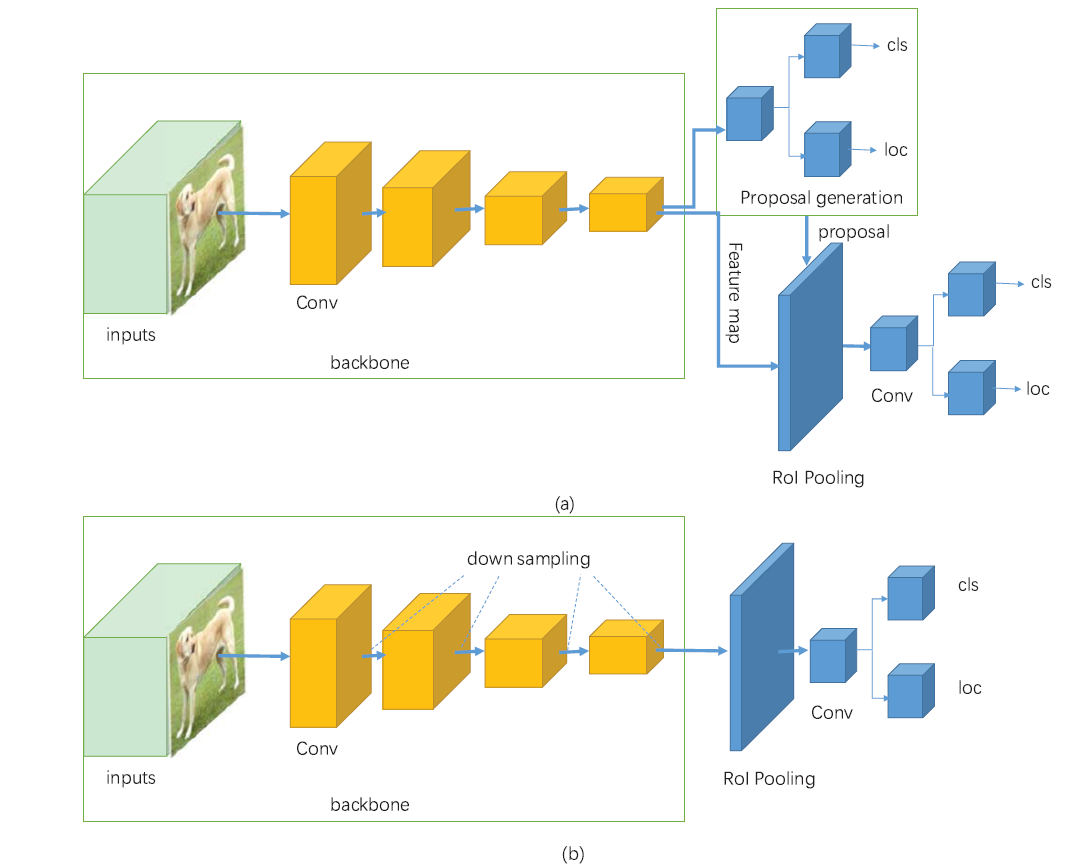
\includegraphics[width=1\linewidth]{images/Object_detector_1stage_vs_2_stage.png}
    \caption{(a) Exhibits the basic architecture of two-stage detectors, which consists of region proposal network to feed region proposals into classifier and regressor. (b) Shows the basic architecture of one-stage detectors, which predicts bounding boxes from input images directly \cite{8825470}.}
    \label{fig:single-two-stage-object-detection}
\end{figure}

Additionally, \textbf{transformer-based object detection algorithms}, such as DETR and RT-DETR, integrate transformers with convolutional neural networks (CNNs) to directly predict object categories and boundaries. This combination enhances efficiency and accuracy, making them a promising choice for modern object tracking applications \cite{zhou2024real}.
\begin{figure}[h]
    \centering
    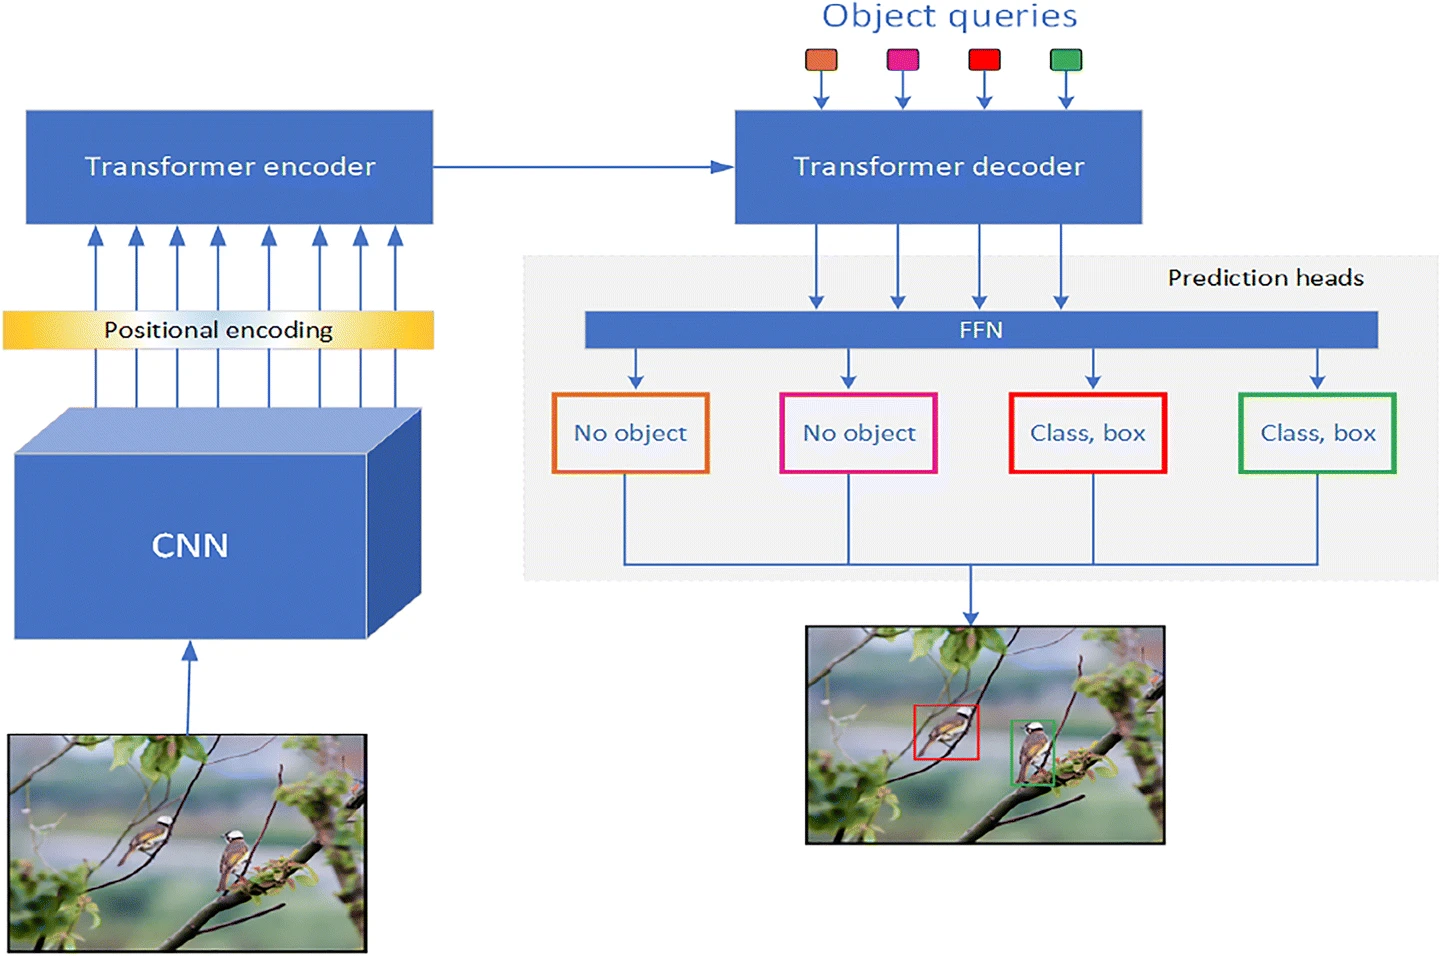
\includegraphics[width=1\linewidth]{images/The process of DETR and its structure.png}
    \caption{The process of DETR and its structure \cite{arkin2023survey}.}
\end{figure}

Despite demonstrating strong performance in terrestrial environments, these algorithms encounter significant challenges in underwater object detection due to factors such as low light conditions and turbid backgrounds \cite{qiu2024boundary}\cite{zhou2024real}\cite{mathias2022occlusion}. Underwater object tracking plays a critical role in applications such as marine resource exploration and military security \cite{qiu2024boundary}. Recent advancements in deep learning have garnered considerable attention for their potential in data-driven underwater image enhancement and object recognition \cite{yang2024lu2net}.

Advanced Deep Learning Techniques Tailored for Underwater Object Tracking (UOT):
\begin{itemize}
    \item \textbf{Knowledge Distillation (KD):} This involves efficiently training a smaller "student" network by learning from a larger, pre-trained "teacher" network. This approach has been applied to UOT, where a teacher model trained on massive open-air data can enhance the tracking performance of a student model dedicated to underwater frames \cite{zhang2024webuot}. Omni-knowledge distillation combines different types of distillation losses, such as token contrastive representation, similarity matrix, feature embeddings, and response maps distillation losses \cite{zhang2024webuot}.
    \item \textbf{Motion-Aware Target Prediction (MATP):} To address model drift caused by similar distractors in underwater environments, a training-free MATP module based on Kalman filtering can be used \cite{zhang2024webuot}. This involves prediction and correction stages to estimate and refine the target's state. UOSTrack also uses motion-based post-processing to mitigate the influence of similar targets \cite{qiu2024boundary}\cite{zhang2024webuot}.
    \item \textbf{Boundary Attention and Sparse Feature Learning:} The DBSF network utilizes a differential boundary attention distribution model to accurately perceive the underwater object edge structure even in noisy and low-resolution images \cite{qiu2024boundary}. It then learns to perceive highly discriminative sparse features on the object structure, reducing the computational demands for edge devices \cite{qiu2024boundary}.
    \item \textbf{Hybrid Training:} Some approaches, like UOSTrack, use hybrid training with both underwater images and open-air sequences to address the sample imbalance problem in underwater datasets \cite{zhang2024webuot}.
    \item \textbf{Siamese network-based trackers}: Siamese networks employ identical neural networks with shared weights to process the target object's initial appearance (template) and subsequent frames (search region) \cite{elmezain2025advancing}. By performing a convolutional feature cross-correlation between these two inputs, Siamese networks learn a similarity function to robustly identify the target across varying conditions and frames \cite{elmezain2025advancing}\cite{zhao2020correlation}\cite{wu2023hybrid}. The tracking task is essentially formulated as a similarity-matching function \cite{wu2023hybrid}.
    \item \textbf{Multi-modal Data:} Leveraging multi-modal data like depth and event information, alongside specialized architectures like multi-scale feature pyramids and transformer-based attention mechanisms, holds significant potential for advancing underwater detection and tracking \cite{elmezain2025advancing}.
\end{itemize}

Deep learning-based object detection models like YOLO, R-CNN, and SSD are used for underwater tracking \cite{lotfi2024comparison}\cite{elmezain2025advancing}. Studies have shown YOLO to be reliable for underwater object detection \cite{lotfi2024comparison}. To enhance temporal stability, YOLO can be merged with SORT \cite{lotfi2024comparison}. Transformer-based architectures are also showing promising results in UOT \cite{mathias2022occlusion}.
\begin{figure}[h]
    \centering
    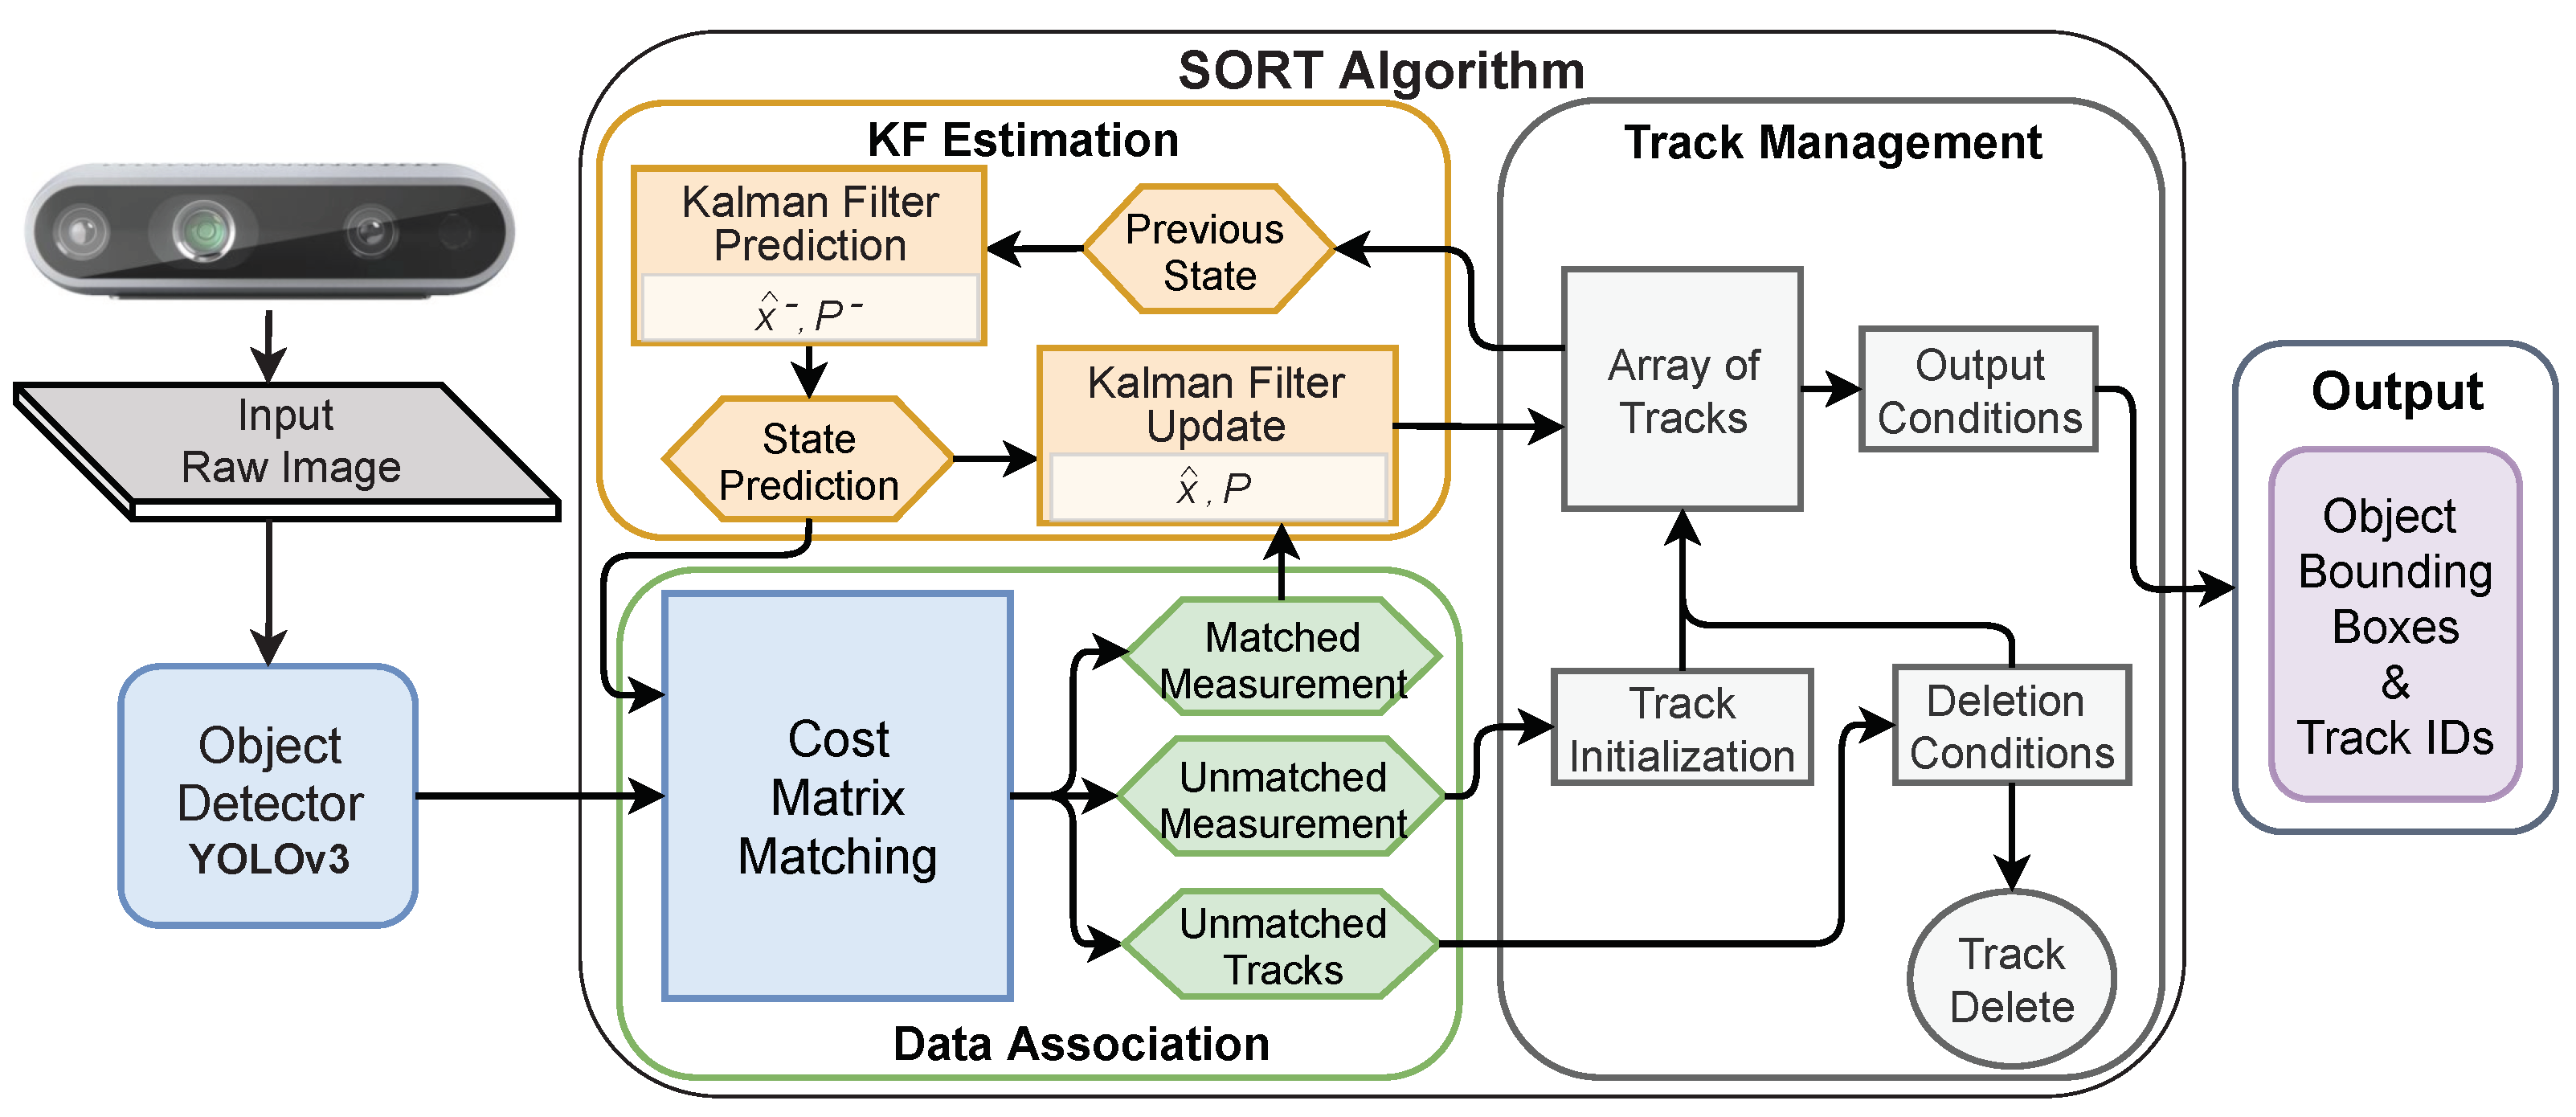
\includegraphics[width=1\linewidth]{images/deepsort.png}
    \caption{Overview of SORT algorithm based YOLOv3 and Kalman filter \cite{pereira2022sort}.}
\end{figure}

% Tracking-by-Detection in Underwater Scenarios:
This paradigm involves using object detection models (like YOLOv3) to detect objects in each frame and then linking these detections across frames using tracking algorithms such as Deep SORT, which can be enhanced with LSTM for handling occlusions, as proposed in the HADSYv3 approach \cite{mathias2022occlusion}\cite{elmezain2025advancing}. This method can be effective in dynamic underwater environments, although its efficacy depends on the quality of the detection algorithm \cite{mathias2022occlusion}.

% dataset and benchmark
Several datasets have been established to promote research in UOT, including UOT32, UOT100, UTB180, VMAT, and UVOT400 \cite{zhang2024webuot}\cite{qiu2024boundary}\cite{rout2019walsh}. However, many lack training sets or have limitations in size and scenario coverage. The WebUOT-1M dataset has been introduced as a larger benchmark to facilitate the development of more powerful deep UOT algorithms \cite{zhang2024webuot}. FishTrack23 is another large-scale dataset specifically for fish tracking \cite{elmezain2025advancing}.

% Performance of Deep Learning Trackers in Underwater Environments:
Evaluations on datasets like WebUOT-1M show that Transformer-based trackers (e.g., OKTrack, UOSTrack, All-in-One, GRM, OSTrack) often perform well \cite{zhang2024webuot}. UOT-specific trackers like OKTrack and UOSTrack, even with plain ViT backbones, can surpass state-of-the-art open-air trackers, highlighting the domain gap between underwater and open-air environments \cite{zhang2024webuot}. Retraining open-air trackers on underwater datasets like WebUOT-1M can effectively reduce this domain gap and improve performance. The DBSF tracker has also demonstrated optimal tracking results on UOT32 and UOT100 benchmarks by focusing on boundary information and sparse confidence features, particularly for edge computing devices \cite{qiu2024boundary}.

% Correlation Filter-Based Tracking Combined with Deep Learning:
Correlation filter (CF) based tracking offers real-time capabilities, and combining it with deep convolutional features has significantly improved performance \cite{qiu2024boundary}\cite{du2021overview}\cite{zhao2020correlation}\cite{lin2024motion}. Algorithms like \textbf{DeepSRDCF}, which uses CNN features, and \textbf{SiamFC}, a fully-convolutional Siamese network, have shown excellent results \cite{zhao2020correlation}. ECO is another efficient correlation filter-based tracker utilizing deep features \cite{zhao2020correlation}\cite{feng2019dynamic}\cite{lin2024motion}. \textbf{MACF} is a motion-aware correlation filter algorithm developed for challenging scenarios like satellite videos with small objects and similar distractors, and it has achieved superior accuracy compared to state-of-the-art trackers \cite{lin2024motion}.

% Challenges and Future Directions in Deep Learning-Based Tracking:
Despite the advancements, challenges remain in UOT, including handling occlusion, small or camouflaged objects, low visibility, optimizing computational efficiency for real-time processing on autonomous systems, and mitigating model drift \cite{qiu2024boundary}\cite{mathias2022occlusion}\cite{zhang2024webuot}\cite{lin2024motion}. Future work includes introducing spatial-temporal features and semi-supervised learning to improve tracking in complex underwater scenes \cite{qiu2024boundary}\cite{mathias2022occlusion}. Enhancing the detection of small or camouflaged objects, optimizing computational efficiency, and improving real-time processing capabilities are also crucial for deployment in autonomous systems \cite{elmezain2025advancing}. For correlation filter-based tracking, future research can focus on designing better filters by considering categorized features, space weight factors, scale factors, and expert strategies, as well as combining manual and deep features \cite{du2021overview}.



%%%%%%%%%%%%%
%%%%%%%%%%%%%
\section{Sensor Fusion-Based Tracking Methods}
Sensor fusion-based approaches in underwater environments leverage data from multiple sensors to enhance surveillance and tracking capabilities \cite{braca2015distributed}\cite{tharmarasa2007large}\cite{uney2022passive}. In contrast to traditional methods that rely on single platforms like submarines or frigates, distributed networks of stationary and mobile sensors, such as autonomous underwater vehicles (AUVs), offer advantages in scalability, robustness, and reliability through intelligent networking \cite{braca2015distributed}. \textbf{Distributed information fusion (DIFFUSION) strategies}, where local information is shared among sensors, are a key aspect of these intelligent networks \cite{braca2015distributed}. This allows for the combination of data from spatially separated sensors to achieve higher performance \cite{braca2015distributed}.

Two primary DIFFUSION schemes are proposed for underwater surveillance: one based on the sharing of local contacts generated by the detection stage, and another based on the sharing of tracks produced by the local tracking stage \cite{braca2015distributed}. In the contact-sharing scheme, contacts are combined at each node using optimal Bayesian tracking based on the random finite set (RFS) formulation \cite{braca2015distributed}. The track-sharing scheme employs a track-to-track (T2T) association and fusion procedure \cite{braca2015distributed}. A local tracker on each AUV provides a set of tracks and their associated covariance matrices, which are then associated and fused with tracks from other AUVs to obtain more accurate state estimates \cite{braca2015distributed}. Unassociated tracks are treated as originating from a single sensor \cite{braca2015distributed}.

The problem of sensor selection within a large network is also critical for optimizing tracking performance under constraints like communication bandwidth \cite{tharmarasa2007large}. Efficient search techniques, such as convex optimization followed by greedy local search, can be employed to determine near-optimal sensor utilization strategies in real-time for multitarget tracking \cite{tharmarasa2007large}. Different approaches to sensor selection include "closest-sensor" strategies, which select sensors nearest to estimated target positions, and more sophisticated methods like "coarse-step" and "fine-step" planning that consider tracking performance over time \cite{tharmarasa2007large}. The posterior Cramér–Rao lower bound (PCRLB) can serve as a basis for network management and as a cost function for optimization \cite{tharmarasa2007large}.

In the context of passive sensor fusion for underwater surveillance, the \textbf{Generalized Labeled Multi-Bernoulli (GLMB)} filter can be used for joint filtering of measurements from multiple sensors, enabling multi-target tracking \cite{uney2022passive}. While detection sets from passive sensors may be staggered in time, the iterated multi-sensor update approach in the GLMB filter has proven sufficiently accurate for simultaneous detections \cite{uney2022passive}. This Bayesian recursion over time allows for long-term integration of sensor data, even when dealing with the non-linearities inherent in bearings-only tracking, often tackled using sequential Monte Carlo methods \cite{uney2022passive}.


\endinput                                     % Вторая глава
\chapter{Theoretical study of algorithms}
\label{ch:fundamental}

In this study, we employ Visual Object Tracking (VOT) methods to address the problem of underwater object tracking. VOT plays a crucial role in tracking objects across video frames, allowing for continuous localization without prior category knowledge. This approach is essential for handling dynamic underwater environments, where objects may undergo significant appearance changes due to lighting variations, occlusions, and water turbulence.

The field of VOT encompasses a diverse range of algorithmic approaches, broadly categorized into traditional correlation filter-based methods and modern deep learning-based techniques. Correlation filter-based trackers leverage frequency-domain operations for efficient tracking [24; 25], whereas deep learning-based methods exploit the representational power of neural networks to enhance robustness against appearance variations and challenging environmental conditions [26; 27]. This section presents a comprehensive theoretical study of key tracking algorithms, providing insights into their underlying principles and methodologies.



\section{Minimum Output Sum of Squared Error (MOSSE)}
The Minimum Output Sum of Squared Error (MOSSE) tracker, introduced by Bolme et al. \cite{bolme2010visual}, represents a pioneering approach in correlation filter-based object tracking. MOSSE employs adaptive correlation filters to efficiently track objects in real-time while maintaining robustness against variations in illumination, occlusions, and background clutter.

\subsubsection{Formulation of MOSSE}
The fundamental objective of MOSSE is to learn an optimal correlation filter $w^*$ that minimizes the sum of squared errors between the actual output of the convolution operation and the desired response, typically modeled as a Gaussian function centered on the target location. The optimization problem is formulated as follows:

\begin{equation} \label{eq:mosse}
    \underset{w^*}{\arg\min} \sum_{i} \left\| f_i \odot w^* - y_i \right\|^2,
\end{equation}
where:
\begin{itemize}
    \item $f_i$ represents the extracted feature map from the $i$-th input frame,
    \item $w^*$ is the correlation filter to be learned,
    \item $y_i$ is the desired response map modeled by a Gaussian function,
    \item $\odot$ denotes element-wise multiplication.
\end{itemize}

\subsubsection{Solution in the Frequency Domain}
Direct computation in the spatial domain is computationally expensive. Leveraging the Convolution Theorem, which states that convolution in the spatial domain is equivalent to element-wise multiplication in the frequency domain, MOSSE reformulates the optimization problem using the Discrete Fourier Transform (DFT):

\begin{equation}
    \hat{w}_i = \frac{\sum_i \hat{y}_i \odot \hat{f}_i^*}{\sum_i \hat{f}_i \odot \hat{f}_i^*},
\end{equation}
where $\hat{\cdot}$ denotes the Fourier transform, and $(\cdot)^*$ represents the complex conjugate.

Once the optimal filter $\hat{w}_i$ is obtained, object localization in a new frame is determined by computing the response map:

\begin{equation}
    \hat{y}_m = \sum_{i=1}^{D} \hat{w}_i \odot \hat{f}_i.
\end{equation}

Applying the inverse Fourier transform recovers the response map in the spatial domain:

\begin{equation}
    y_m = \mathcal{F}^{-1}(\hat{y}_m).
\end{equation}

The target's new location is estimated as the coordinates of the maximum value in $y_m$ \cite{bolme2010visual}.

\subsubsection{Online Filter Update Mechanism}
To account for appearance variations such as lighting changes and partial occlusions, MOSSE employs an online filter update strategy. The filter numerator $A_i$ and denominator $B_i$ are updated adaptively using a learning rate $\eta$:

\begin{equation}
    \begin{aligned}
        A_i &= \eta \hat{y}_i \odot \hat{f}_i^* + (1 - \eta) A_{i-1}, \\
        B_i &= \eta \hat{f}_i \odot \hat{f}_i^* + (1 - \eta) B_{i-1}.
    \end{aligned}
\end{equation}

The updated filter for subsequent frames is computed as:
\begin{equation}
    \hat{w}_i = \frac{A_i}{B_i}.
\end{equation}

This adaptive mechanism enables MOSSE to maintain tracking performance despite dynamic changes in the target's appearance \cite{bolme2010visual}.

\subsubsection{Advantages and Limitations}
MOSSE is well-regarded for its computational efficiency, achieving high-speed tracking rates suitable for real-time applications. Key advantages include:
\begin{itemize}
    \item Robustness to lighting variations and partial occlusions,
    \item Efficient learning with a low computational footprint,
    \item Real-time performance with high frame rates.
\end{itemize}
However, MOSSE has limitations, particularly in handling:
\begin{itemize}
    \item Scale variations, as it assumes a fixed target size,
    \item Background clutter in complex tracking environments,
    \item Non-rigid object deformations.
\end{itemize}

\subsubsection{Conclusion}
MOSSE introduced a groundbreaking framework for object tracking using correlation filters, demonstrating real-time performance with adaptive learning. While its limitations have prompted the development of more advanced trackers, such as Kernelized Correlation Filters (KCF) \cite{henriques2014high}, MOSSE remains a foundational method in visual object tracking due to its simplicity and efficiency.



%%%%% KCF
%%%%%

\section{Kernelized Correlation Filter (KCF)}
The Kernelized Correlation Filter (KCF), introduced by Henriques et al. \cite{henriques2014high}, extends the MOSSE framework by incorporating the kernel trick to project image features into a higher-dimensional space. This non-linear transformation improves the discriminative power of the learned filter, enhancing tracking robustness against appearance variations such as scale changes, deformations, and occlusions \cite{henriques2012exploiting}.

Unlike MOSSE, which operates in the linear domain, KCF utilizes a kernel function $k(x, x')$ that implicitly maps the input data into a high-dimensional feature space without explicit computation. This allows for the use of more complex decision boundaries while maintaining computational efficiency through the use of circulant matrices and the Fast Fourier Transform (FFT) \cite{henriques2014high}.

The optimization problem in KCF follows a similar formulation to MOSSE but extends it using a kernel function:
\begin{equation}
    \underset{\alpha}{\arg\min} \sum_{i} \left\| \sum_{j} \alpha_j k(x_i, x_j) - y_i \right\|^2 + \lambda \|\alpha\|^2,
\end{equation}
where:
\begin{itemize}
    \item $k(x_i, x_j)$ is the kernel function measuring similarity between image patches $x_i$ and $x_j$.
    \item $\alpha$ represents the dual coefficients of the kernel function.
    \item $\lambda$ is a regularization parameter to prevent overfitting.
\end{itemize}

The solution to the above optimization problem in the Fourier domain is given by:
\begin{equation}
    \hat{\alpha} = \frac{\hat{y}}{\hat{k} + \lambda},
\end{equation}
where $\hat{k}$ is the Discrete Fourier Transform (DFT) of the kernelized correlation function \cite{henriques2014high}.

The most commonly used kernel in KCF is the Gaussian kernel:
\begin{equation}
    k(x_i, x_j) = \exp\left(-\frac{\|x_i - x_j\|^2}{2\sigma^2} \right),
\end{equation}
which ensures a smooth response map and improved tracking stability \cite{henriques2012exploiting}.

Once the optimal filter $\hat{\alpha}$ is learned, object localization in a new frame is determined via element-wise multiplication in the Fourier domain:
\begin{equation}
    \hat{y}_m = \hat{\alpha} \odot \hat{k}.
\end{equation}
Finally, the inverse Fourier transform is applied to recover the response map in the spatial domain:
\begin{equation}
    y_m = \mathcal{F}^{-1}(\hat{y}_m).
\end{equation}

The peak value of $y_m$ represents the object's estimated location in the current frame \cite{henriques2014high}.

\subsubsection{Scale Adaptation in KCF}
One limitation of the original KCF tracker is its inability to handle scale variations effectively. To address this, an improved version, known as KCF with scale estimation, introduces a multi-scale search mechanism \cite{danelljan2014accurate}. Instead of relying solely on fixed-size bounding boxes, KCF evaluates different scaled versions of the target appearance and selects the one with the highest response score.

The scale estimation process involves creating a set of scaled versions of the target patch and applying the learned correlation filter to each scale. The optimal scale $s^*$ is selected based on the peak response:
\begin{equation}
    s^* = \arg\max_s \mathcal{F}^{-1}(\hat{\alpha} \odot \hat{k}_s),
\end{equation}
where $\hat{k}_s$ represents the kernelized correlation response at scale $s$. This scale-adaptive mechanism significantly improves tracking performance in scenarios involving object size variations \cite{danelljan2016discriminative}.

\subsubsection{Enhancements in Feature Representations}
The original KCF tracker operates on raw intensity values, but subsequent implementations have incorporated more advanced feature representations, such as:
\begin{itemize}
    \item \textbf{Histogram of Oriented Gradients (HOG)}: Improves robustness to illumination and texture variations \cite{felzenszwalb2010object}.
    \item \textbf{Color Names (CN)}: Enhances performance in scenes with complex backgrounds \cite{danelljan2014adaptive}.
    \item \textbf{Deep Convolutional Features}: Extracted from pre-trained CNNs, allowing for superior target representation \cite{wang2015transferring}.
\end{itemize}
By integrating these features, modern KCF variants achieve significantly higher accuracy and robustness in real-world tracking applications.

\subsubsection{Computational Efficiency and Practical Considerations}
Despite its improvements, KCF remains computationally efficient due to its reliance on FFT and circulant matrix properties. The overall complexity remains $\mathcal{O}(n \log n)$, making it suitable for real-time applications \cite{henriques2014high}. However, practical considerations such as parameter tuning (e.g., regularization weight $\lambda$ and kernel bandwidth $\sigma$) can impact performance, requiring empirical optimization for different datasets \cite{danelljan2015learning}.

\subsubsection{Summary of KCF Improvements}
In summary, KCF extends MOSSE by introducing:
\begin{itemize}
    \item \textbf{Kernel methods} for improved discrimination \cite{henriques2014high}.
    \item \textbf{Scale adaptation} for handling object size variations \cite{danelljan2014accurate}.
    \item \textbf{Advanced feature representations} for better robustness \cite{wang2015transferring}.
    \item \textbf{Computational efficiency} suitable for real-time tracking \cite{henriques2014high}.
\end{itemize}
These enhancements make KCF a widely adopted approach in visual object tracking, balancing accuracy, robustness, and efficiency.



%%%%%%% GOTURN
%%%%%

\section{Generic Object Tracking Using Regression Networks (GOTURN)}
GOTURN, proposed by Held et al.\ \cite{held2016learning}, is a deep learning-based tracker that employs a regression network for fast and robust visual tracking. Unlike correlation filter-based approaches such as KCF, which rely on frequency domain operations, GOTURN formulates tracking as a bounding box regression problem, leveraging a deep convolutional neural network (CNN) to predict object motion from one frame to the next.

Unlike many conventional trackers that perform online adaptation, GOTURN is trained offline on a large dataset of labeled video sequences and images. This enables the tracker to generalize to novel objects at test time without requiring per-sequence fine-tuning \cite{held2016learning}. The model learns a generic mapping between object appearance and motion, making it significantly faster than traditional deep learning-based trackers that involve online learning \cite{held2016learning}.

\begin{figure}[h]
    \centering
    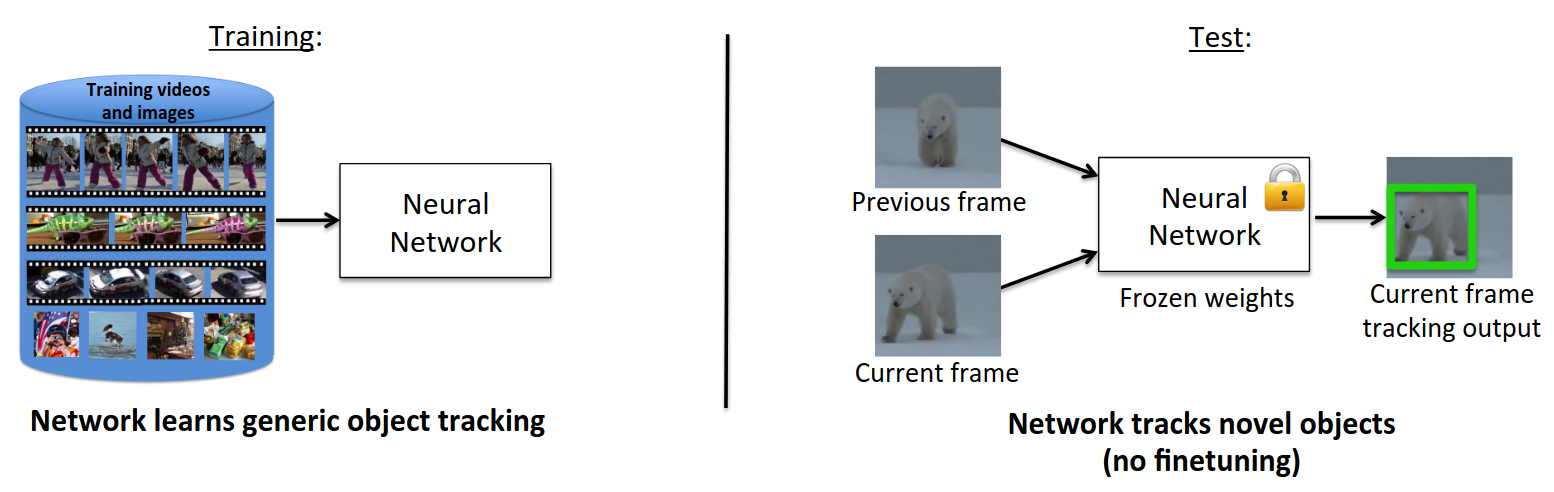
\includegraphics[width=1\linewidth]{images/GOTURN_OVERVIEW.png}
    \caption{A deep neural network is trained using a combination of labeled videos and images to track generic objects. At test time, the network generalizes to unseen objects without requiring fine-tuning, achieving real-time speeds of 100 FPS \cite{held2016learning}.}
    \label{fig:goturn_overview}
\end{figure}

\subsubsection{Network Architecture}
GOTURN consists of a CNN-based regression model that takes as input two consecutive image patches: the search region from the current frame and the target appearance from the previous frame. The network processes these inputs separately through a series of convolutional layers before merging them into a fully connected layer that outputs the coordinates of the tracked object's bounding box in the current frame \cite{held2016learning}.

\begin{figure}[h]
    \centering
    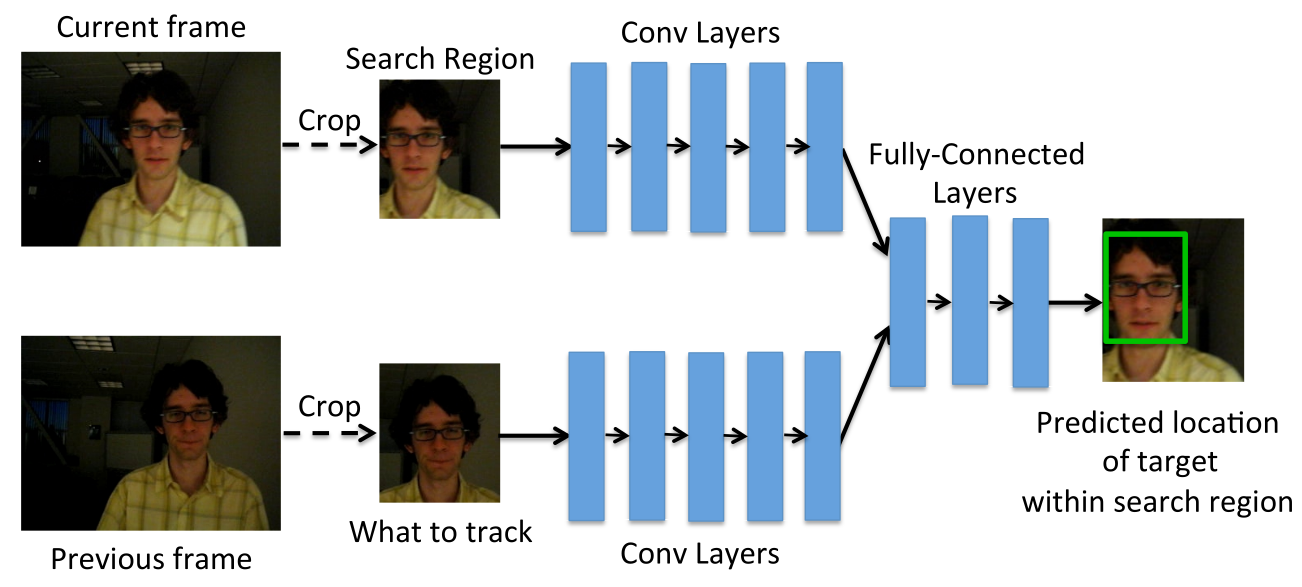
\includegraphics[width=1\linewidth]{images/goturn-architecture.png}
    \caption{The GOTURN architecture \cite{held2016learning}.}
    \label{fig:goturn_architecture}
\end{figure}

The architecture in Picture \ref{fig:goturn_architecture} follows a two-stream design:
\begin{itemize}
    \item The first stream extracts features from the target patch in the previous frame.
    \item The second stream extracts features from the search region in the current frame.
    \item The feature maps from both streams are concatenated and passed through fully connected layers to predict the new bounding box.
\end{itemize}

The convolutional layers are adapted from the CaffeNet architecture \cite{jia2014caffe}, which is a variant of AlexNet \cite{krizhevskyalexnet}. The final regression layer outputs the new bounding box coordinates relative to the search region \cite{held2016learning}.

\subsubsection{Loss Function and Training Strategy}
GOTURN uses an L1 loss function to minimize the difference between the predicted bounding box and the ground truth:
\begin{equation}
    L = \sum_{i=1}^{N} \left| \hat{b}_i - b_i \right|,
\end{equation}
where $b_i$ represents the ground-truth bounding box coordinates, and $\hat{b}_i$ denotes the predicted bounding box.

The network is trained on a combination of labeled video sequences and still images. The video sequences allow the model to learn temporal object motion, while the still images augment the training data by simulating motion via artificial transformations \cite{held2016learning}. The training data is further enhanced using a motion smoothness assumption, where small object movements are favored over large, abrupt changes, improving robustness to motion blur and occlusions.

\subsubsection{Tracking Mechanism}
During inference, GOTURN follows a simple tracking procedure:
\begin{enumerate}
    \item The tracker is initialized with a ground-truth bounding box in the first frame.
    \item For each subsequent frame, a search region centered around the previous bounding box is extracted.
    \item The network predicts the new bounding box coordinates within the search region.
    \item The predicted bounding box is used to update the target location.
\end{enumerate}
This approach allows GOTURN to operate without online fine-tuning, enabling real-time tracking at speeds up to 100 FPS on a GPU \cite{held2016learning}.

\subsubsection{Performance and Limitations}
GOTURN achieves state-of-the-art performance on the VOT-2014 benchmark \cite{held2016learning}, outperforming many traditional trackers in terms of accuracy and robustness. However, its reliance on offline training means it does not adapt to target appearance changes during tracking. Additionally, unlike correlation filter-based trackers such as KCF, it lacks an explicit scale estimation mechanism, making it less effective for tracking objects with large-scale variations \cite{danelljan2016discriminative}.

\subsubsection{Summary of GOTURN Contributions}
GOTURN introduces several key advancements in deep learning-based tracking:
\begin{itemize}
    \item \textbf{Offline training:} Unlike traditional trackers that learn online, GOTURN trains a deep network offline, improving speed and generalization \cite{held2016learning}.
    \item \textbf{Regression-based tracking:} Directly predicts bounding box locations using CNN-based feature extraction and fully connected regression layers \cite{held2016learning}.
    \item \textbf{Real-time performance:} Achieves up to 100 FPS, significantly faster than previous deep learning-based trackers \cite{held2016learning}.
\end{itemize}
Despite its limitations in handling appearance changes and scale variations, GOTURN remains a pioneering approach in deep learning-based object tracking, demonstrating the potential of regression networks for real-time applications.

\section{Siamese Region Proposal Network (SiamRPN)}
Siamese Region Proposal Network (SiamRPN), introduced by Li et al.\ \cite{li2018high}, is an extension of the Siamese network-based tracking framework that incorporates a region proposal network (RPN) for precise and efficient object localization. Unlike GOTURN, which directly regresses bounding box coordinates, SiamRPN applies a matching-based approach where the network learns a similarity function between the target template and candidate regions in the search space.

\subsubsection{Network Architecture}
SiamRPN follows a Siamese network design, consisting of two identical branches that extract deep feature embeddings from the target template and the search region. The key innovation in SiamRPN is the integration of an RPN module, which enables the network to generate multiple object proposals and select the most confident prediction \cite{li2018high}.

\begin{figure}[h]
    \centering
    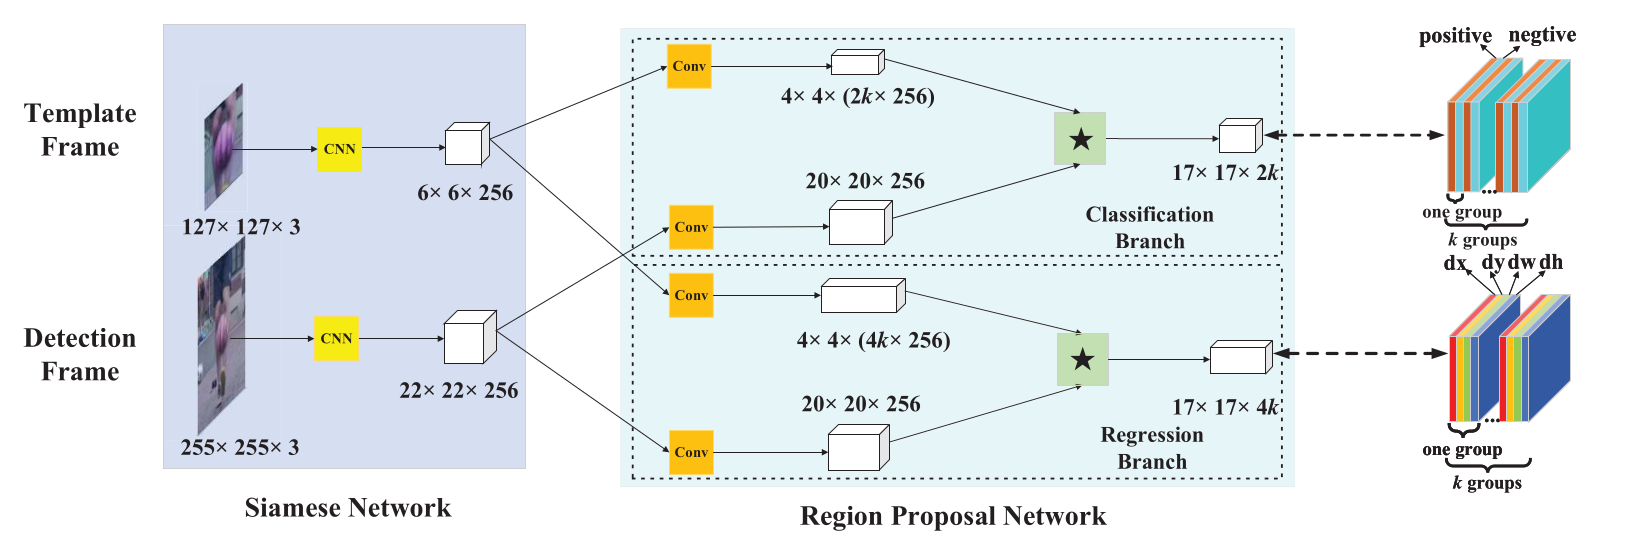
\includegraphics[width=1\linewidth]{images/SiamRPN-architechture.png}
    \caption{The SiamRPN architecture \cite{li2018high}.}
    \label{fig:siamrpn_architecture}
\end{figure}

The network operates as follows:
\begin{itemize}
\item The target template from the first frame is passed through a convolutional backbone (e.g., AlexNet or ResNet).
\item The search region from the current frame is processed through the same backbone.
\item A cross-correlation operation between the two feature maps is performed to compute response maps, representing object similarity.
\item The RPN module generates multiple anchor-based proposals and refines the bounding box predictions.
\end{itemize}
This pipeline enables SiamRPN to perform both localization and classification simultaneously, improving tracking accuracy compared to standard Siamese trackers such as SiamFC \cite{bertinetto2016fully}.

\subsubsection{Loss Function and Training Strategy}
SiamRPN optimizes a multi-task loss function, which includes:
\begin{equation}
L = L_{cls} + \lambda L_{reg},
\end{equation}
where:
\begin{itemize}
\item $L_{cls}$ is the classification loss, typically a cross-entropy loss for distinguishing target vs. background.
\item $L_{reg}$ is the bounding box regression loss, commonly a smooth L1 loss for refining object proposals.
\item $\lambda$ is a weighting factor to balance the two objectives.
\end{itemize}
Training SiamRPN requires large-scale video datasets with ground-truth annotations, such as ImageNet VID and YouTube-BB \cite{li2018high}. The network is pre-trained on static images and fine-tuned on video sequences to learn motion-aware representations.

\subsubsection{Performance and Advantages}
SiamRPN achieves state-of-the-art results on benchmarks such as OTB-2015 and VOT-2018, surpassing traditional trackers in terms of accuracy and robustness \cite{li2018high}. The main advantages of SiamRPN include:
\begin{itemize}
\item High-speed tracking: Runs at over 160 FPS due to efficient network design.
\item Robust localization: RPN improves bounding box estimation.
\item Scale adaptation: Handles object size variations better than fixed-scale trackers.
\end{itemize}
These characteristics make SiamRPN a widely used tracker in real-time applications, including autonomous driving and video surveillance.

\subsubsection{Comparison with GOTURN}
Compared to GOTURN, SiamRPN introduces several key improvements:
\begin{itemize}
\item Matching-based tracking (SiamRPN) vs. regression-based tracking (GOTURN).
\item Anchor-based bounding box proposals vs. direct bounding box prediction.
\item Better scale handling due to multi-scale region proposals.
\end{itemize}
Overall, SiamRPN represents a significant advancement in deep learning-based tracking, combining the efficiency of Siamese networks with the precision of RPN-based object detection.

\subsubsection{Variants of SiamRPN}

Following the success of SiamRPN, several improvements have been proposed to enhance its tracking performance, robustness, and efficiency. These variants introduce modifications to the backbone, region proposal strategy, and feature aggregation techniques.

\textbf{SiamRPN++} \cite{li2019siamrpn++} improves upon SiamRPN by utilizing deeper backbones such as ResNet and introducing spatial-aware sampling strategies to mitigate the limitations of small receptive fields in shallow networks. The network also applies depth-wise separable convolutions to enhance efficiency, making it more robust to large-scale variations.

\textbf{SiamBAN (Balanced Anchor-free Network)} \cite{chen2020siamban} replaces the anchor-based RPN module with an anchor-free mechanism, reducing computational complexity while improving accuracy. Instead of predefined anchor boxes, SiamBAN directly predicts the target’s center location and bounding box size, enhancing adaptability to scale variations.

\textbf{SiamCAR (Classification and Regression)} \cite{guo2020siamcar} further refines the anchor-free tracking paradigm by employing a dense prediction strategy. The network jointly classifies and regresses bounding boxes at each location in the feature map, improving tracking precision while maintaining high speed.

\textbf{LightTrack} \cite{yan2021lighttrack} emphasizes lightweight and efficient tracking by employing neural architecture search (NAS) to design a compact and optimized network. By balancing accuracy and computational efficiency, LightTrack achieves competitive performance while being well-suited for deployment on resource-constrained devices such as mobile and edge platforms.

\textbf{SiamGAT} \cite{lu2023siamese} introduces graph attention networks (GATs) into the Siamese tracking framework, allowing the model to better capture spatial relationships between objects and background features. This enhances tracking performance in cluttered scenes and improves robustness to occlusion.

\section{Transformer Tracker}
Transformer-based models have recently emerged as powerful alternatives to conventional correlation-based tracking frameworks. Unlike traditional approaches such as MOSSE \cite{bolme2010visual} and KCF \cite{henriques2014high}, which rely on handcrafted features and linear correlation, or deep-learning-based methods like SiamRPN \cite{li2018high} and GOTURN \cite{held2016learning}, which incorporate convolutional networks for feature extraction, Transformer-based tracking frameworks leverage self-attention mechanisms to enhance feature fusion and robustness.


\begin{figure}[h]
    \centering
    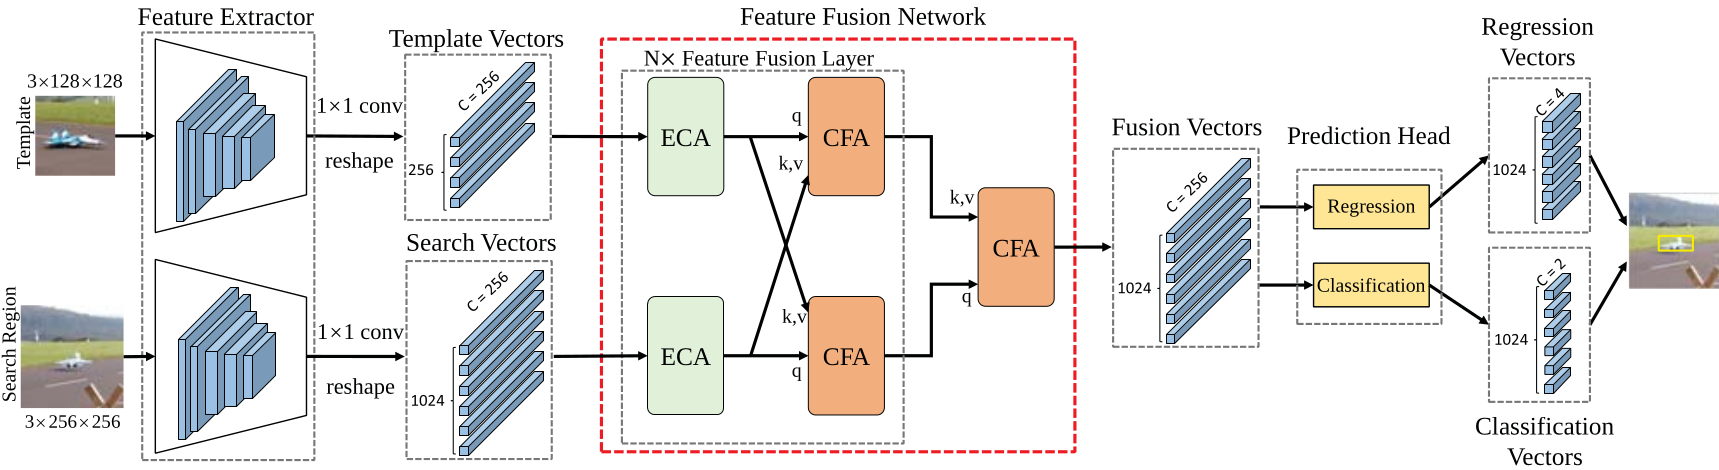
\includegraphics[width=1\linewidth]{images/vitt_architecture.png}
    \caption{Architecture of Transformer tracking framework \cite{chen2021transformer}.}
    \label{fig:transt_architecture}
\end{figure}

\subsubsection{Network Architecture} 
The Transformer architecture, originally proposed for natural language processing \cite{vaswani2017attention}, has been successfully adapted for object tracking. The core idea behind Transformer tracking is the replacement of the conventional cross-correlation operation with an attention-based feature fusion mechanism. One notable example is TransT \cite{chen2021transformer}, which introduces an attention-driven network consisting of an ego-context augment module (ECA) and a cross-feature augment module (CFA). These components effectively enhance global feature interactions between the target template and the search region.


\textbf{Feature Extraction:} Transformer-based trackers typically utilize a Siamese backbone for feature extraction. Given an input template $z \in \mathbb{R}^{3 \times H_z \times W_z}$ and a search region $x \in \mathbb{R}^{3 \times H_x \times W_x}$, a shared feature extractor (often based on ResNet-50 \cite{he2016deep}) processes both inputs to generate feature maps $f_z$ and $f_x$, which are then forwarded to the feature fusion network.

\textbf{Attention-Based Feature Fusion: }Unlike previous methods that apply depthwise cross-correlation for similarity computation, Transformer trackers employ self-attention and cross-attention modules:
\begin{itemize}
    \item \textbf{Ego-Context Augment (ECA):} Enhances local features by capturing long-range dependencies within the template and search region through multi-head self-attention.
    \item \textbf{Cross-Feature Augment (CFA):} Establishes interdependencies between template and search region features, allowing adaptive fusion without explicit correlation operations.
\end{itemize}

% ECA and CFA modules
\begin{figure}[h]
    \centering
    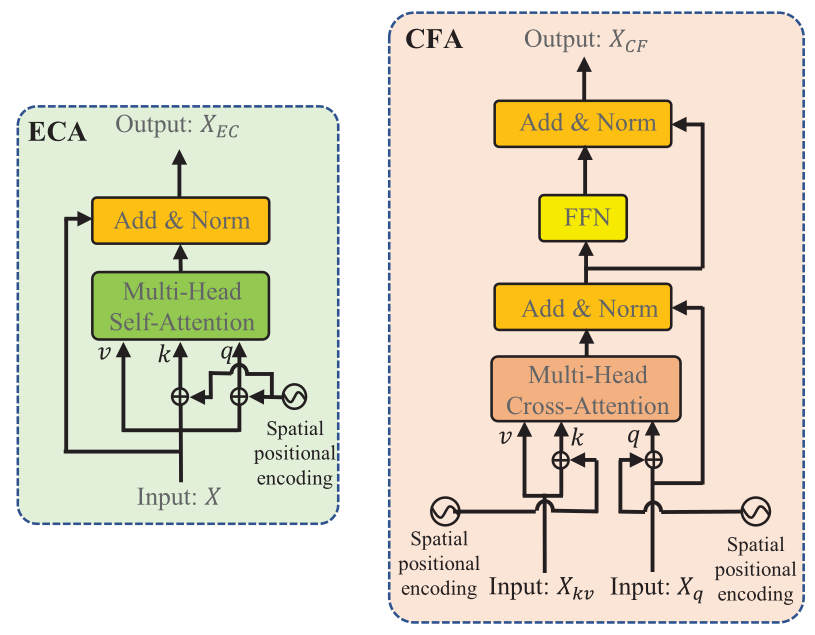
\includegraphics[width=0.8\linewidth]{images/ecs-cfa.png}
    \caption{Ego-Context Augment (ECA) and Cross-Feature Augment (CFA) modules in Transformer tracking \cite{chen2021transformer}.}
    \label{fig:eca_cfa}
\end{figure}

These attention modules enable the tracker to dynamically focus on salient regions of the target, mitigating issues like distractors and occlusion.

\textbf{Prediction Head: }The final stage of the Transformer tracker consists of a classification and regression network that predicts the target's presence and bounding box coordinates. Compared to conventional anchor-based regression techniques used in SiamRPN \cite{li2018high}, Transformer trackers such as TransT \cite{chen2021transformer} adopt a more flexible and parameter-free prediction mechanism, improving robustness against scale variations.

\subsubsection{Loss Function and Training Strategy}
The loss function for Transformer-based tracking is typically a combination of classification and regression losses:
\begin{equation}
L = L_{\text{cls}} + \lambda_{1} L_{\text{IoU}} + \lambda_{2} L_{1}
\end{equation}
where $L_{\text{cls}}$ is the binary cross-entropy loss for classification, $L_{\text{IoU}}$ is the IoU loss for bounding box regression, and $L_{1}$ is the smooth $l_1$ loss. Training is performed using datasets such as LaSOT, GOT-10k, and TrackingNet, with an AdamW optimizer and learning rate scheduling strategies.

\subsubsection{Performance and Advantages}
Transformer-based tracking approaches have demonstrated superior performance on large-scale benchmarks such as LaSOT, TrackingNet, and GOT-10k. Experimental results from \cite{chen2021transformer} indicate that TransT outperforms prior state-of-the-art trackers in terms of Average Overlap (AO) and Success Rate (SR) while maintaining real-time processing speeds (approximately 50 FPS on GPU).

\subsubsection{Comparison with CNN-Based Tracker}
Unlike CNN-based trackers, which rely heavily on handcrafted correlation operations, Transformer trackers leverage self-attention mechanisms that adaptively aggregate features across long spatial distances. This enables improved target localization, especially in scenarios involving occlusion, motion blur, and background clutter. Transformer-based methods also eliminate the need for predefined anchor boxes, leading to a more flexible and efficient tracking pipeline.

\subsubsection{Conclusion}
Transformer-based tracking represents a significant leap forward in visual object tracking, replacing handcrafted correlation operations with adaptive attention mechanisms. The ability to model long-range dependencies and adaptively fuse features makes these models particularly effective in challenging scenarios. Future work may explore hybrid architectures that integrate Transformer attention with convolutional inductive biases to further enhance tracking efficiency and robustness.




\endinput                                     % Третья глава

\printbibliography[title=Список использованных источников] % Автособираемый список литературы

\end{document}